%!TeX TS-program = pdflatex
%!TeX encoding = UTF-8 Unicode
%!TeX spellcheck = en-US
%!BIB TS-program = bibtex
% -*- coding: UTF-8; -*-
% vim: set fenc=utf-8
% inspiration = https://elifesciences.org/articles/34115
% on neural data : https://www.physiology.org/doi/abs/10.1152/jn.00684.2017
%: METADATA
%: %%%%%%%%%%%%%%%%%%%%%%%%%%%%%%%%%%%%%%%%%%%%%%%%%%%%%%%%%%%%%%%%%%%%
\newcommand{\AuthorA}{Chlo\'e Pasturel}
\newcommand{\AuthorB}{Anna Montagnini}%
\newcommand{\AuthorC}{Laurent Perrinet}%
\newcommand{\Address}{Institut de Neurosciences de la Timone, CNRS / Aix-Marseille Universit\'e - Marseille, France}%
\newcommand{\Website}{http://invibe.net/LaurentPerrinet}%
\newcommand{\Email}{Laurent.Perrinet@univ-amu.fr}%
\newcommand{\Title}{
%Principles and psychophysics of Active Inference in anticipating a dynamic probabilistic bias
Should I stay or should I go? Humans adapt to the volatility of visual motion properties, and know about it
%Anticipating a volatile probabilistic bias in visual motion direction
%Humans adapt to the volatility of visual motion properties :  eye movements and explicit guesses
}
\newcommand{\Acknowledgments}{PACE-ITN - code and material @ \url{\Website/Publications/PasturelMontagniniPerrinet2019}. TODO: RIck + Karl + JB + Laurent Madelain }
\newcommand{\Abstract}{
Animal behavior has to constantly adapt to changes, for instance when unexpectedly switching the state of an environmental context. For an agent interacting with this kind of volatile environment, it is important to respond to such switches accurately and with the shortest delay. However, this operation has in general to be performed in presence of noisy sensory inputs and solely based on the currently available information. It has already been shown that human observers can accurately anticipate the motion direction of a visual target with their eye movements when this random sequence of rightward/leftward motions is defined by a bias in direction probability. Here, we generalized the capacity of these observers to anticipate different random biases within random-length contextual blocks. Experimental results were compared to those of a probabilistic agent which is optimal with respect to this switching model. We found a better fit between the behaviorally observed anticipatory response with that of the probabilistic agent compared to other models such as a leaky integrator model. Moreover, we could similarly fit the level of confidence reported by human observers with that provided by the model and derive a common marker for subject inter-variability, titrating their level of preference between exploration and exploitation. Such results provide evidence that in such a volatile environment human observers may still efficiently represent an internal belief, along with its precision, and use this representation for sensorimotor control as well as for explicit judgments. This work proposes a novel approach to more generically test human cognitive abilities in uncertain and dynamic environments.
}
%%%%%%%%%%%%%%%%%%%%%%%%%%%%%%%%%%%%%%%%%%
%\documentclass[profile,final,english,draft,24pt]{article}%
\documentclass[12pt,english]{article}%
\usepackage{fullpage}
% https://www.overleaf.com/learn/latex/Page_size_and_margins
\usepackage[pass]{geometry}
\usepackage{babel}
\usepackage{csquotes}
\usepackage{gensymb}
% MATHS (AMS)
\usepackage{amsmath}
\usepackage{amsfonts}
\usepackage{amssymb}
\usepackage{amsthm}
\newcommand{\KL}[2]{\text{KL}( #1 | #2 )}
%% parenthesis
\newcommand{\pa}[1]{\left( #1 \right)}
\newcommand{\bpa}[1]{\big( #1 \big)}
\newcommand{\choice}[1]{ %
	\left\{ %
		\begin{array}{l} #1 \end{array} %
	\right. }
% ensembles
\newcommand{\ens}[1]{ \{ #1 \} }
\newcommand{\enscond}[2]{ \left\{ #1 \;;\; #2 \right\} }
% egal par définition
\newcommand{\eqdef}{\ensuremath{\stackrel{\mbox{\upshape\tiny def.}}{=}}}
\newcommand{\eqset}{\ensuremath{\stackrel{\mbox{\upshape\tiny set}}{=}}}
\newcommand{\eq}[1]{\begin{equation*}#1\end{equation*}}
\newcommand{\eql}[1]{\begin{equation}#1\end{equation}}
\newcommand{\eqs}[1]{\begin{align*}#1\end{align*}}
\newcommand{\eqa}[1]{\begin{align}#1\end{align}}

\DeclareMathOperator{\argmin}{argmin}
\DeclareMathOperator{\argmax}{argmax}
\newcommand{\uargmin}[1]{\underset{#1}{\argmin}\;}
\newcommand{\uargmax}[1]{\underset{#1}{\argmax}\;}
\newcommand{\umin}[1]{\underset{#1}{\min}\;}
\newcommand{\umax}[1]{\underset{#1}{\max}\;}
\newcommand{\usup}[1]{\underset{#1}{\sup}\;}
% for units
\usepackage{siunitx}%
\newcommand{\ms}{\si{\milli\second}}%

%% Symboles arrondis
\newcommand{\Aa}{\mathcal{A}}
\newcommand{\Bb}{\mathcal{B}}
\newcommand{\Cc}{\mathcal{C}}
\newcommand{\Dd}{\mathcal{D}}
\newcommand{\Ee}{\mathcal{E}}
\newcommand{\Ff}{\mathcal{F}}
\newcommand{\Gg}{\mathcal{G}}
\newcommand{\Hh}{\mathcal{H}}
\newcommand{\Ii}{\mathcal{I}}
\newcommand{\Jj}{\mathcal{J}}
\newcommand{\Kk}{\mathcal{K}}
\newcommand{\Ll}{\mathcal{L}}
\newcommand{\Mm}{\mathcal{M}}
\newcommand{\Nn}{\mathcal{N}}
\newcommand{\Oo}{\mathcal{O}}
\newcommand{\Pp}{\mathcal{P}}
\newcommand{\Qq}{\mathcal{Q}}
\newcommand{\Rr}{\mathcal{R}}
\newcommand{\Ss}{\mathcal{S}}
\newcommand{\Tt}{\mathcal{T}}
\newcommand{\Uu}{\mathcal{U}}
\newcommand{\Vv}{\mathcal{V}}
\newcommand{\Ww}{\mathcal{W}}
\newcommand{\Xx}{\mathcal{X}}
\newcommand{\Yy}{\mathcal{Y}}
\newcommand{\Zz}{\mathcal{Z}}
%% ========  polices de caracteres =============
\usepackage[T1]{fontenc}%
\usepackage{lmodern}%
\usepackage{t1enc}
\usepackage{ragged2e}
%============ graphics ===================
\usepackage[pdftex]{graphicx}%
\DeclareGraphicsExtensions{.pdf,.png,.jpg}%
\graphicspath{{./figures/}}% TODO remove {./figures/},  at the end
%============ bibliography ===================
%\usepackage[numbers,comma,sort&compress,round]{natbib} %
\usepackage[
%style=alphabetic-verb,
style=authoryear-comp,
%style=apa,
%maxcitenames=2,
%maxnames = 2,
giveninits=true,
uniquename=init,
sorting=none,
url=false,
isbn=false,
eprint=false,
texencoding=utf8,
bibencoding=utf8,
autocite=superscript,
backend=bibtex,
%articletitle=false
]{biblatex}%
%\addbibresource{Pasturel_etal2018.bib}%
\bibliography{Pasturel_etal2019.bib} % the ref.bib file
\newcommand{\citep}[1]{\parencite{#1}}
\newcommand{\citet}[1]{\textcite{#1}}
%%%%%%%%%%%%%%%%%%%%%%%%%%%%%%
%% OPTIONAL MACRO FILES
\usepackage{tikz}
%\usepackage{tikz,tkz-euclide} \usetkzobj{all} % loading all objects
%\usetikzlibrary{positioning} \usetikzlibrary{calc}
%\usepackage{sfmath}
\newcommand{\seeFig}[1]{Figure~\ref{fig:#1}}
\newcommand{\seeEq}[1]{Equation~\ref{eq:#1}}
\newcommand{\seeApp}[1]{Appendix~\ref{app:#1}}
\newcommand{\seeSec}[1]{Section~\ref{sec:#1}}
%============ hyperref ===================
\usepackage[unicode,linkcolor=red,citecolor=red,filecolor=black,urlcolor=red,pdfborder={0 0 0}]{hyperref}%
\hypersetup{%
pdftitle={\Title},%
pdfauthor={\AuthorA},%< \Email > \Address},%
}%
\usepackage{color}%
\newcommand{\LP}[1]{\textbf{\textcolor{red}{[LP: #1]}}}
\newcommand{\AM}[1]{\textbf{\textcolor{blue}{[AM: #1]}}}
\newcommand{\CP}[1]{\textbf{\textcolor{green}{[CP: #1]}}}

\usepackage{listings}
\usepackage{color}

\definecolor{dkgreen}{rgb}{0,0.6,0}
\definecolor{gray}{rgb}{0.5,0.5,0.5}
\definecolor{mauve}{rgb}{0.58,0,0.82}
%============ code ===================
\usepackage{listings}
\lstset{frame=tb,
  language=Python,
  aboveskip=3mm,
  belowskip=3mm,
  showstringspaces=false,
  columns=flexible,
  basicstyle={\small\ttfamily},
  numbers=none,
  numberstyle=\tiny\color{gray},
  keywordstyle=\color{blue},
  commentstyle=\color{dkgreen},
  stringstyle=\color{mauve},
  breaklines=true,
  breakatwhitespace=true,
  tabsize=3
}
%%%%%%%%%%%%%%%%%%%%%%%%%%%%%%%%%%%
\title{\Title}%
\author{\AuthorA,
\AuthorB,
\AuthorC\thanks{\Address} }

%%%%%%%%%%%% Her begynner selve dokumentet %%%%%%%%%%%%%%%
\begin{document}%
\maketitle%
%%%%%%%%%%%%%%%%%%%%%%%%%%%%%%%%%%%%%%%%%%%%%%%%%%%%%%%%%%%%%%%%
%: Abstract
\begin{abstract}
\Abstract
\end{abstract}
%: %%%%%%%%%%%%%%%%%%%%%%%%%%%%%%%%%%%%%%%%%%%%%%%%%%%%%%%%%%%%%%%
\section{Motivation}
%%%%%%%%%%%%%%%%%%%%%%%%%%%%%%%%%%%%%%%%%%%%%%%%%%%%%%%%%%%%%%%%
\label{sec:intro}
%%%%%%%%%%%%%%%%%%%%%%%%%%%%%%%%%%%%%%%%%%%%%%%%%%%%%%%%%%%%%%%%
%%%%%%%%%%%%%%%%%%%%%%%%%%%%%%%%%%%%%%%%%%%%%%%%%%%%%%%%%%%%%%%%
\subsection{Volatility of sensory contingencies and
the adaptation of cognitive systems}
% SUMMARY : cognition adaptation to volatility
% ------------------------------------------------------------------
% * the evolution  of prices on the stock market: Any Socio-economic contextual index may make the price evolve up or down, slowly or more Rapidly
% * ecological change
% * the side (left or right of the field) in which the ball is on a soccer field
% \LP{Anna, I found a better example which was less dramatic than ``
% Think for instance of the variability of environmental contingencies
% present in global climate and
% the probability of a change in its dynamic
% since the switch of civilization in an industrialized organization:
% We have access to (possibly noisy and heterogeneous) measurements
% of some (few) markers, such as carbon dioxide concentration and
% wish to predict the range of the mean temperature on Earth.
% This reveals some of the dynamics of
% the complex system constituted by the atmosphere
% and of acceptable levels of temperature for civilization.
% Based on past history and prior knowledge about
% the effect of our own emissions of carbon dioxide
% (for instance priming evidence of the link between carbon dioxide
% concentration and an elevation of temperature),
% one should be able to predict at best if either
% one could continue to exploit a similar strategy (emit gases)
% or if it is necessary to explore different paradigms (limit emissions).
% '' Hope you like it :-) }
% \AM{ I like the green example too: it only demands to define the variable that would correspond to the time series to be tracked: carbon dioxide measurements at a given critical location? Also, the fact that a switch detection may inform important decision is nice for the example but we do not really have an analogy to it in our task. Yet I am very happy with both examples, both very much on fashion, are we more ecology, or pro-vax activists?!}
%: general volatility and perceptual learning
We live in a fundamentally volatile world for which
our cognitive system has to constantly adapt.
Imagine for instance you are a doctor (general practitioner) and
that you usually report an average number of
one person infected by measles per month.
On the past few days however,
the rate increased to four cases per week.
As such, two alternate interpretations are available:
Either, there is an outbreak of measles and
one should estimate its incidence
(as measured as the rate of new cases)
since the onset of the outbreak.
Alternatively, these cases are
``unlucky'' coincidences that originate from the volatility
of a genuinely stationary and heterogeneous random process
that underly and generated these observations.
In that option, it may be possible to readjust
the estimated baseline rate of infection with this new data.
This example illustrates one fundamental problem
with which our cognitive system is faced:
when observing new sensory evidence,
\emph{should I stay} and continue to integrate this novel data
to my current beliefs about the environment's state
or \emph{should I go} and adopt a new hypothesis
about the random process generating the observations
since the detection of a switch in the environment?

Such \emph{meta-analysis} of the environmental statistical properties is an effective strategy at the large scale level of our example,
but also at all levels which are behaviorally relevant,
such as contextual changes in our everyday life.
Inferring near-future states in a dynamic environment, such that one can prepare to act upon them ahead of their occurrence~\citep{PerrinetAdamasFriston2014} ---
or at least forming beliefs as precise as possible
about a future environmental context ---
are ubiquitous challenges for cognitive systems.
In the long term, how the human brain manages
the trade-off between exploitation and exploration
is essential to the adaptation
of the behavior through reinforcement learning~\citep{Cohen2007}.
In controlled experimental settings challenging visual perception or sensorimotor associations,
such adaptive processes have been mostly put in evidence
by precisely analyzing the participants' behavior in a sequence of experimental trials,
typically highlighting sequential effects
at the time scale of one to several minutes.
% TODO: talk about Gallistel / Sugrue / Brody

%: Past history of sensory event integration in vision
Indeed, stimulus history of visual events influences
how current stimuli are perceived~\citep{Sotiropoulos2011, Adams12} and acted upon~\citep{Carpenter1995, Maus2015,Damasse18}.
Two qualitatively opposite effects of the stimulus history have been described, priming and perceptual adaptation. Adaptation reduces
the sensitivity to recurrently presented stimuli and
thus to re-calibrate perceptual experience~\citep{Clifford2007, Webster2011, Kohn2007}.
Examples of negative biases in perceptual discrimination are
numerous~\citep{REFFS} and show that the visual system tends
to favor temporal and spatial stability of the stimulus:
On the other hand, priming is a facilitatory effect that
enhances the identification of repeated stimuli~\citep{Verstraten1994, Tiest2009}.
This type of perceptual learning leads to improvements in discrimination
with long-term training on a perceptual judgment~\citep{Lu2009}.
In sensorimotor control,
the same stimulus presented several times could indeed
lead to faster and more accurate responses and,
on the other hand, lead to critically suboptimal behavior
when a presented stimulus is not coherent
with the participant's expectations~\citep{Hyman1953, Yu2009}.
This process is highly dynamic especially in complex environments
where new contingencies can arise at every moment.
Overall, the ability to detect
statistical regularities in the event sequence
thus appears as a fundamental ability
for the adaptive behavior of living species.
Very few studies have addressed the question of whether
the estimate of such regularities is explicit,
and whether verbal reports of the dynamic statistical
estimates would eventually correlate to the measures of behavioral adaptation. Here we aim at investigating this question in the specific case of motion direction processing.
In addition, we attempt to palliate to the lack of a solid modeling approach to best understand the computation underlying behavioral adaptation to the environment's statistics,
and in particular how sequential effects are integrated
within a hierarchical statistical framework.
At present, Bayesian inference offers an effective methodology
to deal with this question.

%: Bayesian methods & role of predictive processing for this adaptive response
% TODO : clarify this paragraph
In all generality, Bayesian methods allow to define and quantitatively assess
a range of hypotheses about the processing by some formal agents
of (possibly noisy) information~\citep{Deneve1999, Diaconescu2014, Daunizeau10a}.
A key principle in the Bayesian inference approach is
that each stated hypothesis is quantitatively formalized
using a generative model for the input / output response function
by defining a graph of dependencies between defined variables.
It then follows that measurements and outcomes may be linked by
generic probabilistic computations.
The generative model is parameterized by structural variables
(such as weights, non-linear gain functions or prior knowledge)
and transforms some relevant latent variables
which may be represented as probabilities.
Then, using the rules of probability calculus
one can progressively update beliefs about the latent variables,
such that one can finally infer the hidden structure of received inputs~\citep{Hoyer2003, Ma2014}.https://www.overleaf.com/project/5c36121f4b0f20641e21e49d
For instance, using Bayes's rule, one can combine
the likelihood of observations given the generative model and
the prior of these latent variables~\citep{Janes2014}.
Of particular interest for us is the possibility to
quantitatively represent
the predictive and iterative nature of the probabilistic model.
Indeed, once the belief about latent variables
is formed from the sensory input,
this belief can be used to update
the prior over future beliefs on latent variables~\citep{Montagnini2007}.
Thus, the comparisons between expectations and actual data produces
constant updates to the estimates of the model and
is formalized in all generality within the~\textit{active inference} framework~\citep{Friston2003, Friston2010}.
In summary, Active Inference allows to predict latent variables
but also to understand longer time effects such as adaptation and learning.

In a recent study,~\citet{Meyniel16} simulated a model
over five previously published datasets~\citep{Squires1976, Huettel2002, Kolossa2013, Cho2002, Falk1997}.
Their main conclusion was that
a learning of local transition probabilities
was sufficient to explain the large repertoire
of experimental effects reported in these studies.
They concluded that transition probabilities constitute
a core building block of sequence knowledge in the brain,
which then applies to a variety of sensory modalities and
experimental situations.
As such, sequential effects in binary sequences are better explained
by a learning of transition probabilities
than of the absolute item frequencies or the frequencies of their alternations.
The critical difference lies in the content
of what is learned (transition probabilities versus item frequencies)
in an attempt to capture human behavior.
%TODO say it is an optimization that is, a measure of the dynamic compromise between exploration and exploitation
%Chopin and %Mamassian and the use of visual confidence  (see Ann rev of Vision 2016)
Interestingly, the observation of priming effects
have also been observed for anticipatory smooth eye movements (aSPEM)
and therefore allow to further deepen our understanding of such predictive processes. %
%As a consequence, Bayesian inference allows to compare the explanatory power
%of different models...

% ------------------------------------------------------------------
\subsection{Anticipatory Smooth Pursuit Eye Movements (aSPEM)}
% ------------------------------------------------------------------
% SUMMARY : particular case of aSPEM
%-------------------------------------------------------------%
%: FIGURE 1A fig:intro ~\seeFig{intro}
\begin{figure}%[b!]
\centering{
%\includegraphics[width=\linewidth]{figure1}
\begin{tikzpicture}%[thick,scale=1, every node/.style={scale=1} ]
\node [anchor=north west]  (imgA) at (0.000\linewidth,.600\linewidth){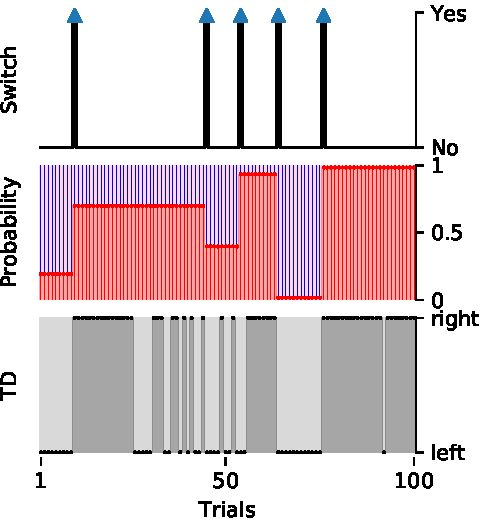
\includegraphics[width=0.325
\linewidth]{1_A_Experiment_randomblock}};
\node [anchor=north west]  (imgB) at (0.340\linewidth,.580\linewidth){\includegraphics[width=0.450\linewidth]{1_B_protocol_recording}};
\node [anchor=north west]  (imgC) at (0.810\linewidth,.511\linewidth){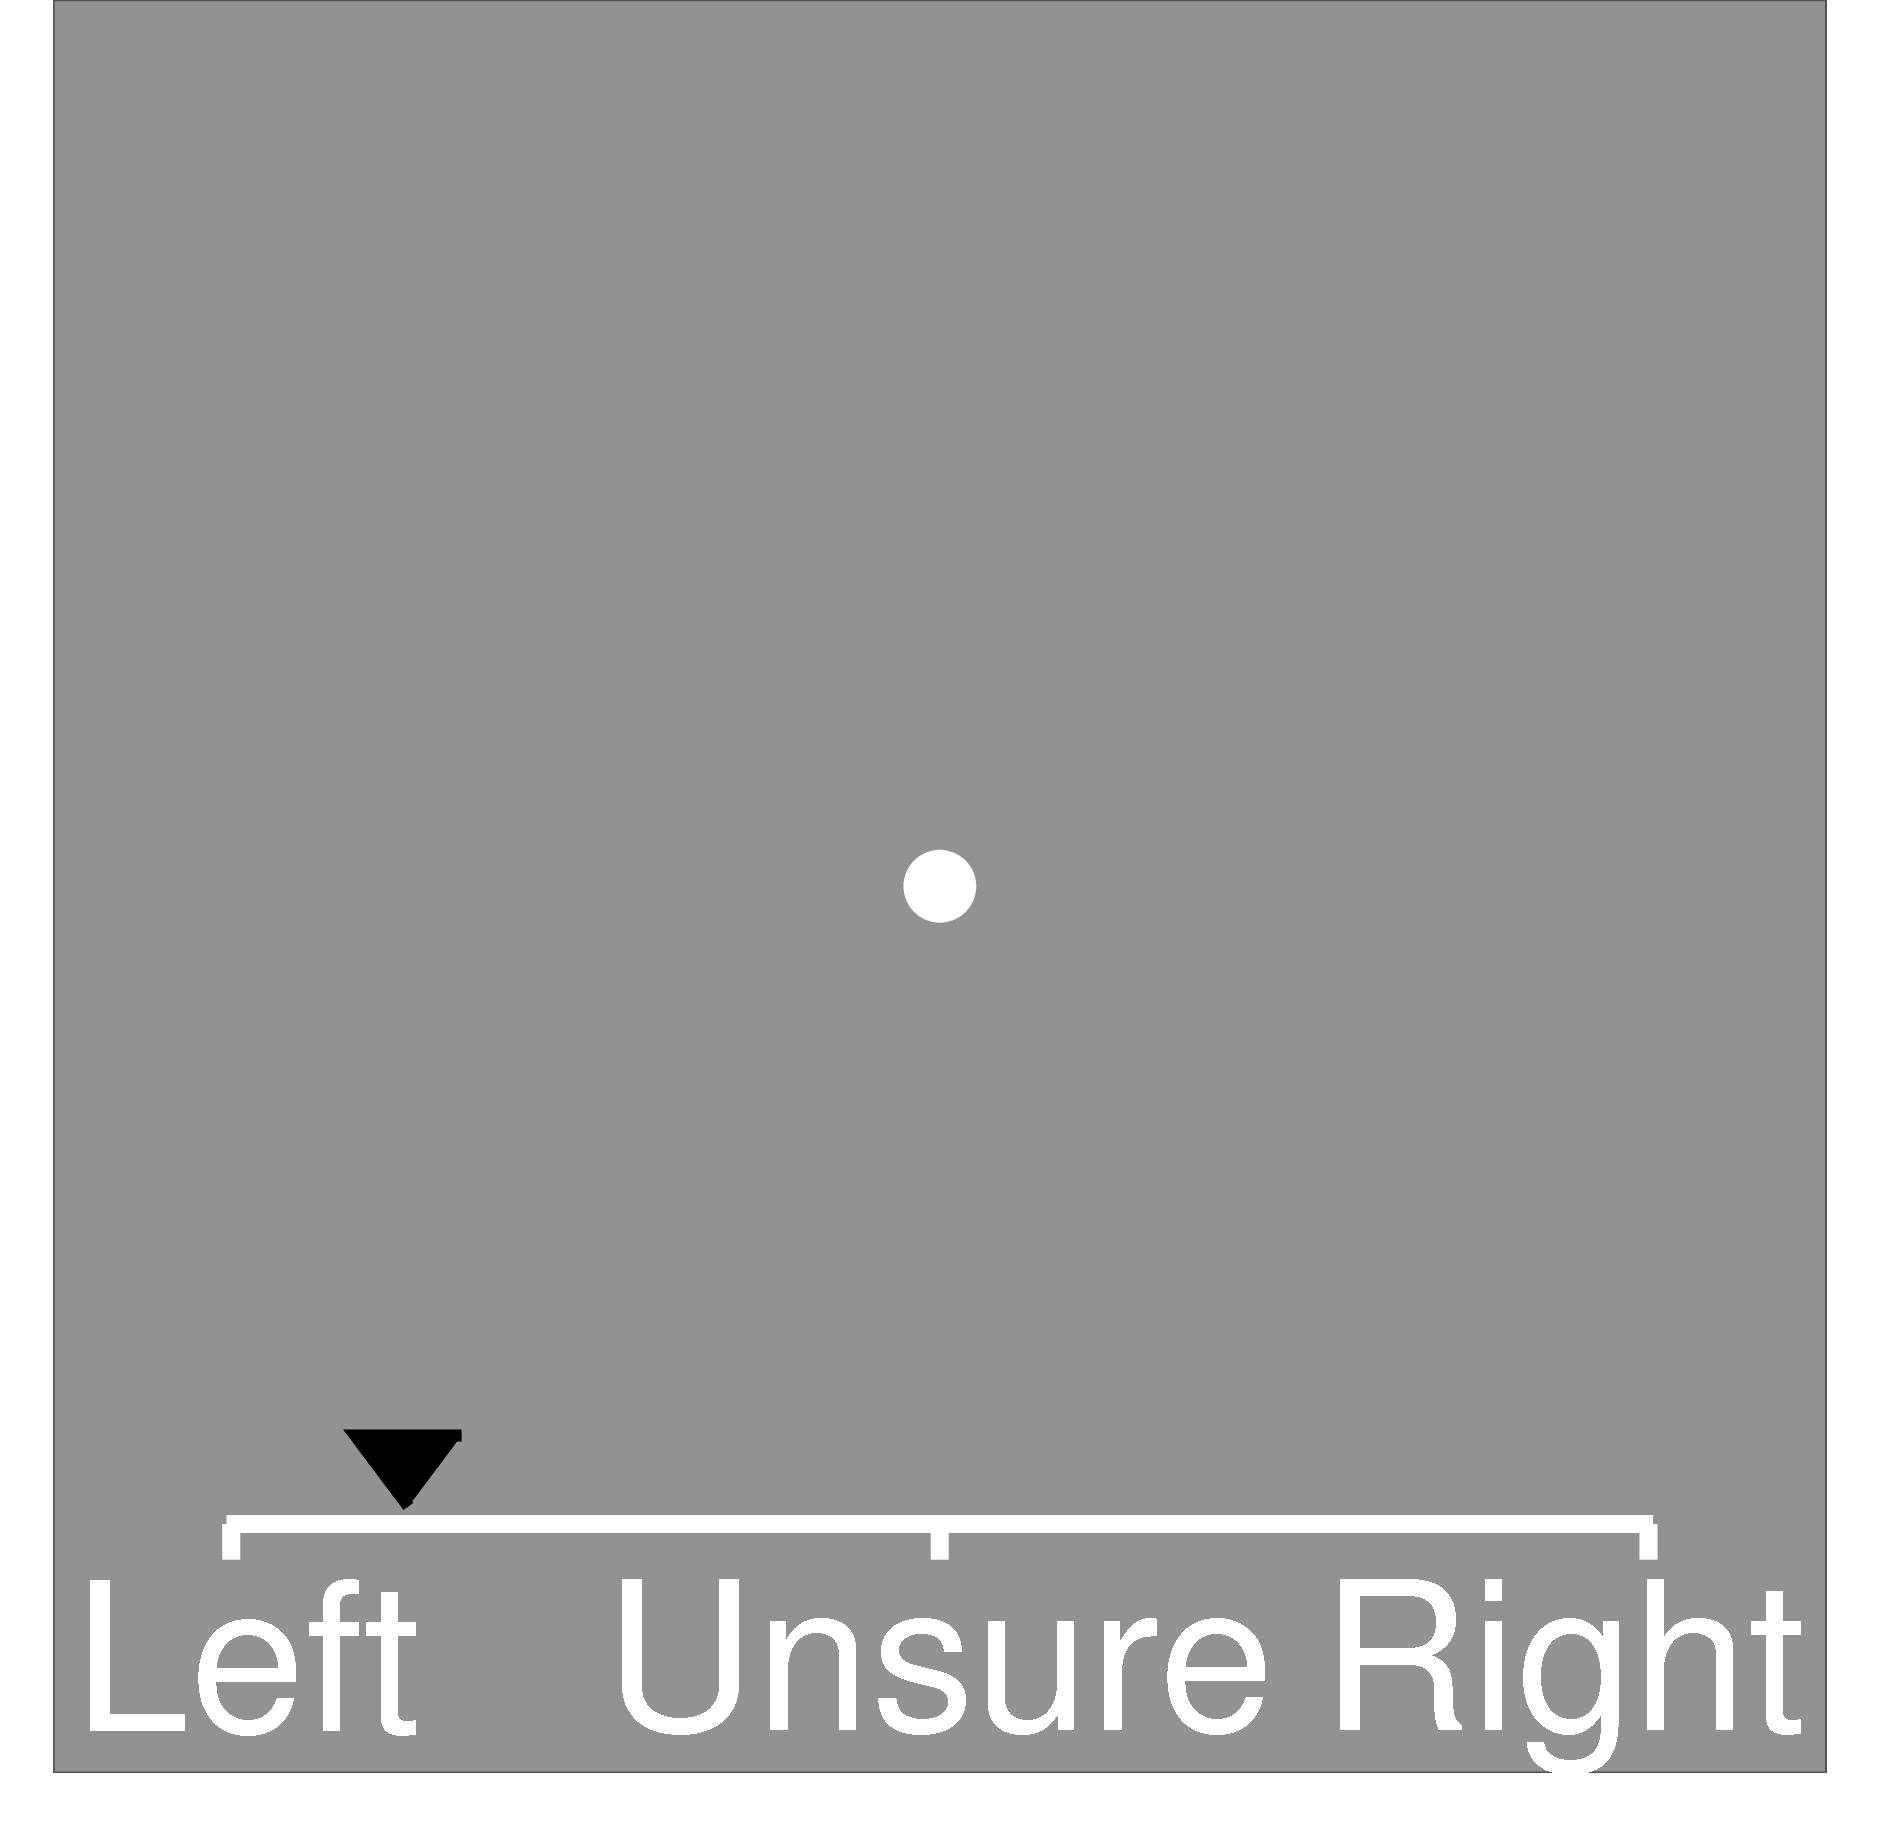
\includegraphics[width=0.145\linewidth]{1_C_protocol_bet_simple}};
\draw [anchor=north west] (0.000\linewidth, .62\linewidth) node {$\mathsf{(A)}$};
\draw [anchor=north west] (0.330\linewidth, .62\linewidth) node {$\mathsf{(B)}$};
\draw [anchor=north west] (0.802\linewidth, .62\linewidth) node {$\mathsf{(C)}$};
\end{tikzpicture}
}
\caption{
\emph{Tracking eye movements and confidence rating in a volatile switching environment}
\textbf{(A)}~
We tested the capacity of human subjects to adapt to a volatile environment 
by using a simple, 3-layered generative model of fluctuations in target directions (TD).
This binary variable is chosen using a Bernoulli trial of a given probability bias.
This probability is itself chosen at random from a given prior 
and is constant for as many trials until a switch is generated.
Switches are generated in the third layer as a Bernoulli trial 
with a given hazard rate (defined here as $1/40$ per trial).
\textbf{(B)}~
The eye-movements task was an adapted version of a task developed by~\citet{Montagnini2010}. 
Each one of $600$ trials consisted of sequentially:
a fixation dot (of random duration between $400$ and $800$~\ms),
a blank screen (of fixed duration of  $300$~\ms) and
a moving ring-shaped target (with $15~\degree/s$ velocity) which the observers were instructed to follow.
The direction of the target (right or left) was drawn pseudo-randomly
according to the generative model defined above. 
\textbf{(C)}~In order to titrate the adaptation 
to the environmental volatility of target direction at the conscious level,
we invited each observer to perform a new variant of the direction-biased experiment on a subsequent day,
where we asked participants to rate, before each trial, the level of confidence
for their estimate of the forthcoming direction of the target.
As shown in this sample screenshot,
this was performed by moving a mouse cursor on a continuous rating scale
between ``sure left'', to ``unsure'' and finally ``sure right''.
}
\label{fig:intro}
\end{figure}
%-------------------------------------------------------------%
%: adaptation to volatility in EMs : seen as an anticipation in SPEM - principle and function
Humans are able to accurately track a moving object
with a combination of saccades and
Smooth Pursuit Eye Movements (SPEM)~\citep{ref}.
These movements allow us to align and
stabilize the object on the fovea,
thus enabling high-resolution visual detection.
This process is retarded by different factors such as axonal transduction,
neural processing and the inertia of the oculomotor system~\citep{Krauzlis89}.
When predictive information is available about target motion,
anticipatory SPEM (aSPEM) are
efficiently generated before target's appearance~\citep{Westheimer1954, Kowler1979a, Kowler1979b} thereby reducing visuomotor latency.
Moreover, some experiments have demonstrated the existence
of prediction-based smooth pursuit during
the transient disappearance of a moving target~\citep{Badler2006,BeckerFuchs1985}.
Overall, although the initiation of SPEM is almost always driven by a visual motion signal, it is now clear that smooth pursuit behavior
can be modulated by extra-retinal, predictive information even in the absence of a direct visual stimulation.
The anticipatory smooth pursuit behavior is remarkable
in different aspects.
First, its buildup is relatively fast, such that only a few trials are sufficient
to pick up some regularity in a binary sequence of alternating Right-Left directions.
Second, it is in general an unconscious process
of which participants are not aware of.
As such, this behavior is a \AM{potentially a useful marker
to study the internal representation of motion expectancy (or Prior) and in particular to analyze} how sensorimotor expectancy interacts dynamically with contextual contingencies in shaping (oculomotor) behavior.

%: linear relationship (talk about santos & kowler and others)
Typically, aSPEM is observed after a temporal cue and
ahead of target motion onset~\citep{Kowler1979a,Kowler1979b, Kowler1984}. %~(see \seeFig{intro}-A).
It is generally assumed that the role of anticipatory eye movements is
to minimize as fast as possible the visual impairment due
to the amplitude of eye-to-target position and velocity mismatch.
\AM{I WOULD POSTPONE THIS SENTENCE SOMEWHERE ELSE, AS IT IS DISTRACTING HERE... The compromise between speed and accuracy is shaped
by the variability introduced by the neural noise
at the neuro-motor junction~\citep{Harris98}.}
Overall, this reduces the typical sensorimotor delay
between target motion onset and foveation~\citep{REFNEEDED}.
In a previous study~\citep{Montagnini2010},
we have analyzed how forthcoming motion properties,
such as target speed or direction, can be
predicted and anticipated with coherently oriented eye movements~(see \seeFig{intro}-A).
It has been observed that the strength of anticipation,
as measured by the mean anticipatory eye velocity,
increases when the target repeatedly moves in the same direction~\citep{Kowler1984, Kowler1989, Heinen2005}.
We similarly found a graded effect of both the speed and the direction-bias
on the strength of aSPEM (see \seeFig{intro}-B).
In particular, this effect is linearly related
to the probability of motion's speed or direction~(see \seeFig{intro}-B).
These results are coherent within previous oculomotor findings
by our and also other groups~\citep{SantosKowler2017}.
These results imply that the probability bias over a target's direction is
one additional factor beyond other physical and cognitive cues~\citep{Kowler2014, SantosKowler2017,Damasse18}
that modulate the common predictive framework
driving anticipatory behavior to optimize a rapid and
precise foveation of the target on its expected future path.

%: limits of the previous method
In order to generalize such results to more ecological conditions,
it is necessary to extend the experimental protocol of~\citet{Montagnini2010} in three aspects.
First, it seems important to investigate the integration of environmental statistical regularities
in this smooth tracking task with
a large family of direction-biases for the target motion.
As such, instead of a finite set of probability biases, % ($.25$, $.5$, $.75$, $.9$ and $1.$, see \seeFig{intro}-B),
we decided to use a continuous range of probability biases~$p$.
%which we were sampling from a fixed prior distribution.
Second,~\citet{Maus2015} have recently shown that
both perceptual adaptation for speed estimation
and priming of aSPEM could occur simultaneously.
They found a robust repulsive adaptation effect
with perceptual judgements biased in favor of faster percepts
after seeing stimuli that were slower and~\textit{vice-versa}. \AM{Concurrently, these authors also found
a positive effect on anticipatory smooth pursuit, with faster anticipation after faster stimuli.}
Indeed, both priming and adaptation can hypothetically share
a common internal representation of stimulus' speed,
reasonably built according to the mean velocity of the last observed movements.
The comparison of the internal representation of speed
with the current stimulus velocity could explain repulsive aftereffects and,
at the same time, be used to elicit
an aSPEM component at the appropriate velocity
for next stimulus occurrences.
\citet{Maus2015} estimated the past history effects over different times scales,
with the priming effects being maximized
for short stimulus histories (around $2$ trials) and
adaptation for longer stimulus history, around $15$ trials.
Their main conclusion was that
perceptual adaptation and oculomotor priming
are the result of two distinct readout computational processes using the same internal representation of motion regularities.
Both these history lengths can be considered
short in comparison to the several hundreds
of trials that are commonly used in psychophysics and sensorimotor adaptation studies.
% ------------------------------------------------------------------
\subsection{Contributions}%Outline}
% SUMMARY : what is novel in our work
% ------------------------------------------------------------------
%: how we do it : or rather why we do it this way (and not like Matthys)
The goal of this study is to generalize the adaptive process
observed in the aSPEM response to more ecological settings but
also to broaden its scope by showing that such unconscious process
also occurs at the conscious level.
To analyse the effect of history length in all generality,
we therefore extended the protocol such that the probability bias
is fixed in sub-blocks with variable block lengths.
%The equations for this protocol will be detailed below~(\seeSec{bayesian_change_point}).
Indeed, by manipulating the probability for target motion direction,
as measured during a fixed duration gap
before target ramp-motion onset~(see \seeFig{intro}-A),
it is possible to bias the direction and mean velocity of aSPEM~(see \seeFig{intro}-B).
This suggests that probabilistic information may be used
to inform the internal representation of motion prediction
for the initiation of anticipatory movements~\citep{Montagnini2010}.
However, it is yet unclear what method to use
to dynamically manipulate the probability of the input sequence.

First, one possible confound in the previous study
is that the range of possible biases is finite and
that there is no direct experimental evidence that
any continuous value within the possible range (that is, the segment $[ 0, 1 ]$)
may be picked up by the visual system.
Second, another possible caveat comes from the fact that the sequence of blocks of conditions on $p$
was used within blocks of fixed lengths.
Indeed, observers may potentially pick up
the information on this fixed length
to predict the occurrence of switches in conditions.

Additionally, we observed qualitatively that following the switch from
one condition to the next,
the strength of aSPEM changed gradually,
consistently with other adaptation paradigms~\citep{Fukushima1996,Kahlon1996,Souto13},
but for which the adaptation mechanism was only fitted.
As a consequence, such estimate may become particularly
challenging in a dynamic context,
where the probabilistic contingencies vary in time in an unpredictable way.
In addition, whether and how the information processing underlying
the buildup of aSPEM and its dynamics is linked to
an explicit estimate of probabilities is unknown.
To alleviate this problem, we developed a new paradigm
in order to address this question
by explicitly modeling a dynamic process with a given volatility:
In particular, our design will make sure that one can manipulate the variable $p$
as a function of trial number by making $p$ itself a random variable. %,
% but also that we can devise an ideal observer for each sequence of inputs.
% TODO check transition
In order to understand the nature of the representation of motion regularities underlying eye movement adaptive behavior, it is crucial to collect verbal explicit judgments about expectations on motion direction, in addition to the recording of eye movements.
In such an explicit judgment task, we evaluated for each participant their confidence for the next trial direction
(\emph{prior} to the appearance of the target).
%on a rating scale
%between "sure left", to "unsure" and finally "sure right"~(see \seeFig{intro}-C).


%\subsection{Generative model: the binomial switching model}
%-------------------------------------------------------------%
%%%: FIGURE 2 fig:results_raw ~\seeFig{results_raw} 
%%% cf 1_generative-model.ipynb
%%\begin{figure}%[b!]
%%\centering{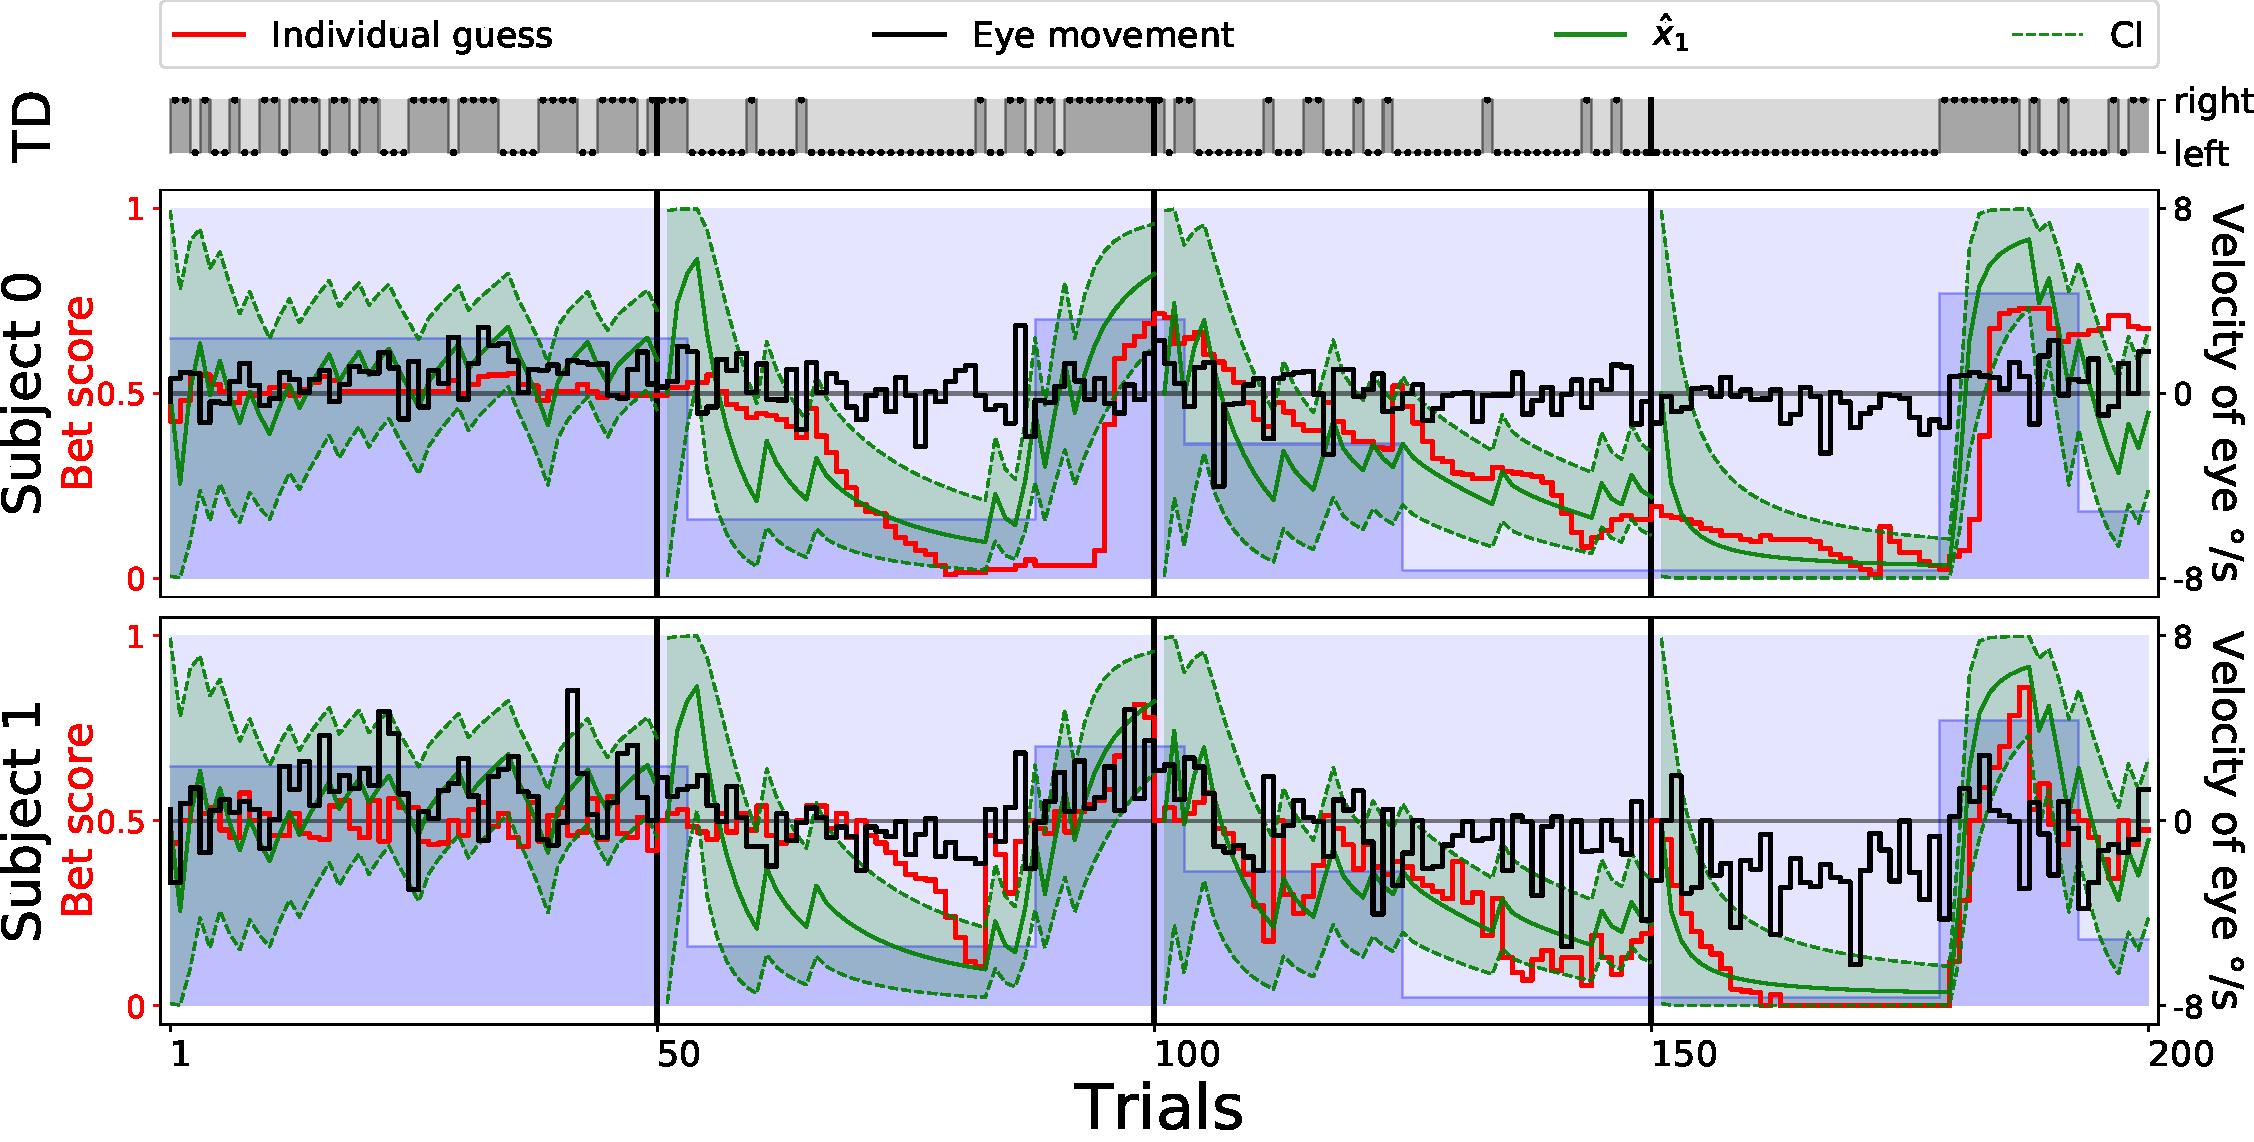
\includegraphics[width=\linewidth]{2_results_enregistrement}}
%%\caption{
%%\emph{Raw behavioral results.} %
%%The top row represents the sequence of target directions (TD)
%%that were presented to observers
%%for one block of $200$ trials
%%as generated by the binomial switching model (see~\seeFig{intro}-A).
%%The bottom rows show the raw behavioral results 
%%for two representative observers.
%%We have overlaid 
%%1/ the recorded aSPEM strength as measured by the horizontal eye velocity estimated right before
%%the onset of the visually-driven SPEM (black line);
%%these values were here scaled according to their extremal values,
%%2/ the bet score as given by the rating scale (red line),
%%3/ the evolution of the value 
%%of the probability bias $p$ used to generate the TD sequence (red shaded areas)
%%and which are hidden to the observers.
%%Qualitatively, one can observe a trend with the polarity of aSPEM velocity
%%to be negative for $p$ values below~$.5$ and positive for values above~$.5$.
%%In addition, the explicit bet score
%%for the next trial's motion direction
%%seems to follow a similar trend.
%%Both curve seem to lag of few trials 
%%after the occurrence of a switch
%%(also hidden to the observers).
%%Note that we introduced short pauses every $50$ trials (as denoted by vertical black lines), to prevent from fatigue and check for possible drifts of the recorded eye position.
%%}
%%\label{fig:results_raw}
%%\end{figure}
%%%-------------------------------------------------------------%
%: design of the binomial switching generative model
Indeed, to assess the dynamics of the adaptive processes
which compensate for the variability of sensory sequences,
one may generate random sequences for the value of $p$,
with a parametric mechanism controlling for the volatility at each trial.
By definition, volatility measures the temporal variability
of the sufficient parameters of a random variable.
% \AM{THEN I HAVE A QUESTION: GIVEN THIS DEFINITION, DOES VOLATILITY CHANGE AT EACH TRIAL IN OUR CASE, OR IS VOLATILITY FIXED ONCE THE TAU=40 PARAMETER HAS BEEN CHOSEN?} it is given by tau /on average/
In the \emph{Hierarchical Gaussian Filter} model (HGF, ~\citet{Mathys11}) for instance,
volatility is controlled as a non-linear transformation
of a random walk (modeled itself by a Brownian motion with a given diffusion factor).
This hierarchical model allows to ultimately generate a sequence of binary choices
where the variability fluctuates along a given trajectory.
Such a forward probabilistic model is invertible
using some simplifying assumptions and allows
to extract an inference of the agent's belief about volatility~\citep{Vossel14}.
Herein, we will use a simpler model where
the bias $p$ in target direction varies according to a piecewise-constant function
%(that is, a step function varying between~$0$ and~$1$),
similarly to~\citet{Meyniel13}.
Indeed, within each sub-block, the volatility of the value of $p$
progressively decreases as we accumulate samples.
It means that instead of a complex stochastic trajectory,
we draw random events (that we denote as ``switches'')
with a given mean frequency,
and that the bias in target direction is stationary between two switches:
The value $p$ of the bias only changes at the moment of a switch,
independently of the previous bias' value.
Such a sequence is presented in ~\seeFig{intro}-A, %TODO : add A + blue line
where we show the realization of the target's directions sequence, and
the trajectory of the underlying (hidden) probability bias.

% equations
Mathematically, this can also be considered as a three-layered hierarchical model
defining the evolution of the model for each trial $t$ as the vector  $(x_2^t, x_1^t, x_0^t)$.
At the topmost layer,
the occurrence $x_2^t \in \{ 0, 1 \}$ of a switch ($1$ for true, $0$ for false)
is  drawn from a Bernoulli process with the switch's frequency $1/\tau$ as the main parameter.
The value of $\tau$ thus gives the average length (in number of trials)
between the occurrence of two switches.
The probability bias $p$ in target direction is a random variable that we define as $x_1^t \in [0, 1]$.
It is chosen at random from a prior distribution $\Pp$ at the moment of a switch,
and else it is constant until the next occurrence of a switch.
Finally, a target moves either to the left or to the right,
and we denote this variable (target direction) as $x_0^t \in \{ 0, 1 \}$.
This direction is drawn from a Bernoulli process $\Bb$
parameterized by the direction bias $p=x_1^t$.
Mathematically, this is easily described
by a 3-layered graphical model according to %~(\seeFig{results_psycho}-A) and
the following equations:
\begin{itemize}
    \item Occurrence of a switch: $x_2^t \propto \Bb(1/\tau)$
    \item Dynamics of probabilistic bias: \eql{\choice{\text{if} \quad x_2^t=0 \quad \text{then} \quad  x_1^t = x_1^{t-1} \\
\text{else} \quad x_1^t \propto \Pp  }\label{eq:bsm}}
    \item Sequence of directions:  $x_0^t \propto \Bb(x_1^t)$
\end{itemize}
% \eql{\choice{
% x_2^t \propto \Bb(1/\tau) \\
% % TODO: nest the choice
% \choice{\text{if} \quad x_2^t=0 \quad \text{then} \quad  x_1^t = x_1^{t-1} \\
% \text{else} \quad x_1^t \propto \Pp  \\
% } \\
% x_0^t \propto \Bb(x_1^t)
% }\label{eq:bsm}}
Note that the prior distribution $\Pp$ can be for instance
the uniform distribution $\Uu$ on $ [ 0, 1 ] $ or
Jeffrey's prior $\Jj$~(see \seeApp{bcp}).
There is always a switch at $t=0$ (that is, $x_2^0=1$). \AM{In addition, we imposed a switch to occur after $200$ and $400$ trials, in order to be able to compare adaptation properties across different chunks of the trials sequence.
The model generating the experimental sequence of trial directions, as well as the experimental protocol are illustrated in~\seeFig{intro}. With a three-layers structure, the model generates the randomized occurrence of the switches,
the length of sub-blocks with constant direction probability
(chosen in the continuous range of possible bias' values), and finally the random sequence of trial direction occurrences?
In conclusion, the system of three equations~\seeEq{bsm}
defines the Binomial Switching Model (BSM)
which we used for the generation of experimental sequences presented to human participants in the experiments,
but also as the basis of an ideal observer model.}

%: outline
This paper is organized in five parts.
After this introduction where we presented the motivation for this study,
the next section~(\seeSec{bayesian_change_point}) will present
an inversion of the BSM forward probabilistic model,
coined the Binomial Bayesian Change Point (BBCP) model.
To our knowledge, such algorithm is not available yet, and
we will here provide it with an analytical solution,
by extending previous results from~\citet{AdamsMackay2007}
to the case of binomial data as in the BSM presented above.
In addition, this solution is \emph{online},
that is, that all computations on the sequence may be done
using solely the variables available at the present trial,
compactly representing all history see in previous trials.
We will also provide a computational implementation
and a quantitative evaluation of this algorithm.
Then, in~\seeSec{results_psycho} we will present the analysis of experimental evidence
to validate the generalization of previous results %.
%In a first session, participants observe a target moving horizontally
%with constant speed from the center
%either to the right or left across trials
with this novel protocol. %~(see \seeFig{intro}-A \& B).
Such results will allow us to fit the inverse model and to compare
its prediction compared to classical models such as the leaky integrator model.
%The probability of either motion direction changes randomly in time.
While in a first session, we recorded anticipatory eye movements, 
in a second experimental session, participants were asked to estimate
``how much they are confident that
the target will move to the right or left in the next trial'' and
to adjust the cursor's position on the screen accordingly~(see \seeFig{intro}-C).
These results will be compared to the results for eye movements.
Similarly, we will show that these results fit well
with the inverse model.
In~\seeSec{inter}, we will synthesize these results
by inferring the volatility parameters extracted
for each individual participant. % and session.
This will allow the analysis of inter-individual behavioral responses for each session
and in particular if one could predict observers' prior volatility,
that is, a measure of the dynamic compromise between exploration (``should I stay?'')
and exploitation (``should I go?'')
across the two different sessions testing predictive adaptive processes
at the unconscious and conscious levels.
Finally, we will summarize and conclude this study and
offer some perspectives for future work in~\seeSec{outro}.
%: %%%%%%%%%%%%%%%%%%%%%%%%%%%%%%%%%%%%%%%%%%%%%%%%%%%%%%%%%%%%%%%
\section{Results: Binomial Bayesian Change Point (BBCP) model}
%%%%%%%%%%%%%%%%%%%%%%%%%%%%%%%%%%%%%%%%%%%%%%%%%%%%%%%%%%%%%%%%
%%%%%%%%%%%%%%%%%%%%%%%%%%%%%%%%%%%%%%%%%%%%%%%%%%%%%%%%%%%%%%%%
\label{sec:bayesian_change_point}
%%%%%%%%%%%%%%%%%%%%%%%%%%%%%%%%%%%%%%%%%%%%%%%%%%%%%%%%%%%%%%%%
%
%: short intro
%
As we saw above, Bayesian methods provide with
a powerful framework for studying human behavior.
In the HGF model~\citep{Mathys11}, for instance,
authors defined a multi-layered generative model for
sequences of input stimuli.
By ``inverting'' this stochastic forward process,
one could extract relevant descriptors at the different levels of the model
and fit these parameters with the recorded behavior.
Here, we will use a similar approach but on a different generative model,
as defined in~\seeEq{bsm}.
First, we will define a first ideal observer as a control
which assumes that volatility is stationary with a fixed frequency.
Then, we will extend it by modeling an agent
which assumes the existence of switches, that is,
that the value of the probabilistic bias may change
at specific (yet randomly drawn) trials,
as was modeled by the forward probabilistic model defined in~\seeEq{bsm}.
%
% ------------------------------------------------------------------
\subsection{Forgetful-agent model (Leaky integrator)}%
% ------------------------------------------------------------------
%: justification from previous studies
Following~\citet{Maus2015},
we modeled a first ideal observer,
which represents a classical, widespread and
realistic model of how trial-history shapes
adaptive processes in human behavior.
It is adapted to model motion expectation in a direction-biased experiment.
In this model, the temporal evolution of the expectation $p=x_1^t$ of a given event
can be modeled by making a simple heuristic:
the update of the estimated probability for an event is based
on the discount of the previously estimated probability
by a factor $1 - h \in [0, 1]$, relative to new information~\citet{Anderson2006}.
At trial $t$, this model can be expressed with the following equation:
\eql{
\hat{x_1}^{t} = (1 - h) \cdot \hat{x_1}^{t-1} + h \cdot x_0^t
\label{eq:leaky}}
where $\hat{x_1}^{t=0}$ is equal to some prior value ($.5$ in the unbiased case),
thjat is for the best guess before observing any data.
% NOTE: it's an AR(1) process https://stats.stackexchange.com/questions/358162/writing-ar1-as-a-ma-infty-process

%: from heuristics to ideal observer
The estimated probability $\hat{x_1}^{t}$ is computed
from the integration of previous instances
with a progressive discount of past information.
The value of the scalar $h$ represents
a compromise between responding rapidly
to changes in the environment ($h \approx 1$) and
not prematurely discarding information still of value
for slowly changing contexts  ($h \approx 0$).
In the following, we will call this scalar the hazard rate.
Equivalently, one can define $\tau = 1 / h$ as
a characteristic time (in units of number of trials)
for the integration of information.
Looking more closely at this expression,
the ``forgetful agent'' computed in \seeEq{leaky}
consists of an exponentially-weighted moving average (see \seeApp{leaky}).
It may thus be equivalently written in the form of a moving average:
\eql{
\hat{x_1}^{t} = h \cdot \sum_{0\leq i \leq t} (1 - 1/\tau)^{i} \cdot x_0^{t-i}
\label{eq:leaky2}}
% \AM{In principle there should also be a term proportional to $(1-h)^{t}$$\hat{x_1}^{t=0}$, true? Which tends to $0$ for large $t$...}
% \LP{it's the term for $i=t$ - ok?}
Inversely, let us assume that at each trial,
the true probability bias changes randomly with a rate of once
every $\tau$ trials.
As a consequence, the probability that the bias does not change is $Pr(x_2^t=0)=1-1/\tau$ at each trial.
Assuming independence of these occurrences, the estimated probability $p=\hat{x_1}^{t}$ is thus the sum
of the past observations weighted by the belief that the bias has not changed during $i$ trials in the past, that is, exactly as defined in~\seeEq{leaky2}.
This shows that
assuming that changes occur at a constant rate ($\hat{x_2}^t=h$)
but ignoring the temporal occurrence of the switch,
the optimal solution to this inference problem is the
ideal observer defined in~\seeEq{leaky2},
which finds an online recursive solution in~\seeEq{leaky}.
We therefore proved here that the heuristic derived from~\citet{Anderson2006}
is an ideal inversion of the generative model
which assumes a fixed average duration for the probability bias.
% \AM{It seems to me that the main limit of this ideal observer is that it is lazy: it knows that on average things change every tau trials but it does nothing to actively estimate and account for these changes: maybe we should have a sentence here to introduce this concept of "active"/"adaptive" observer?} - LP : right, ours is indeed a more active agent, but that's quite subjective...

%: using \hat{p} as a regressor
The correspondence that we proved between the weighted moving average heuristic
and the ideal observer model as a solution to that generative model leads
us to several interim conclusions.
First, the time series of inferred $\hat{x_1}^{t}$ values can serve as a regressor
to test whether human observers follow a similar strategy.
In particular, one could test the free parameter $\tau$,
relative to the agents' belief in the weight decay:
Importantly, $\tau$ may be fitted to the experimental data
that would be collected.
%for instance to the data shown in~\seeFig{results_intro}.
However, one should be careful with such conclusions whenever
this trajectory is fitted to behavioral data.
For instance, if the inversion of the forward model is exact in the present case,
one has to use approximations in more complex models,
such as with the HGF~\citep{Mathys11}
or with the models developed by~\citet{Wilson13,Wilson18}.
As a result, some discrepancy could originate from these approximations
at the algorithmic level.
As such, it is essential that these both sources of discrepancy (intrinsic versus extrinsic)
should be controlled independently~\citep{Beck12}.
Second, if we assume that the inversion of the model is perfect
(that is, that no algorithmic approximation has been done in the inferrence),
this means that by fitting different ideal observers
to the data, one evaluates as a matter of fact the adequacy of
a generative model, not to probabilistic calculus.
This is a common confusion around the idea of a ``Bayesian brain''.
We believe here that the challenge is not to validate the hypothesis that the brain uses or not the Bayes' theorem,
but rather to test different hypotheses
about the different generative models
that agents may use.
This methodological point may be essential in designing the experimental protocol,
or in evaluating quantitatively the results.

%: limits of the leaky integrator
Now, since we have defined a first generative model
and the ideal observer which it corresponds to,
we will define a more complex model
in order to overcome some of the limits of the leaky integrator.
Indeed, a first criticism could be that
this model may be too rigid and does not sufficiently
account for the dynamics of volatility~\citep{Behrens07}
or Bayesian uncertainty~\citep{Vilares2011}.
It seems plausible that the memory (history length) the brain uses
for inference is varying and that this variation could be related
to the volatility inferred from information in the past.
The model presented in~\seeEq{leaky2} uses a constant weight
(decaying with the distance to the current trial)
for all trials, while precision of each trial
can be potentially evaluated and used
for precision-weighted estimation of the probability bias.
To address this hypothesis, our next model will be inspired
by a Bayesian Change-point detection model~\citep{AdamsMackay2007},
which models an ideal agent inferring
both the trajectory of the probability bias ($x_1^t$)
and the probability $Pr(x_2^t=1)$ of the occurrence of switches.
% ------------------------------------------------------------------
\subsection{Binomial Bayesian Change Point model}
% ------------------------------------------------------------------
%-------------------------------------------------------------%
%: FIGURE 3 fig:bayesianchangepoint \seeFig{bayesianchangepoint}
\begin{figure}%[b!]   
% cf 3_Results_2.ipynb
\centering{
\begin{tikzpicture}[thick,scale=.95]
\node [anchor=north west]  (imgA) at (0.000\linewidth,.580\linewidth){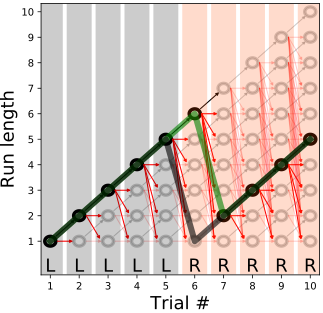
\includegraphics[width=0.382
\linewidth]{3_BCP_model}};
\node [anchor=north west]  (imgB) at (0.382\linewidth,.580\linewidth){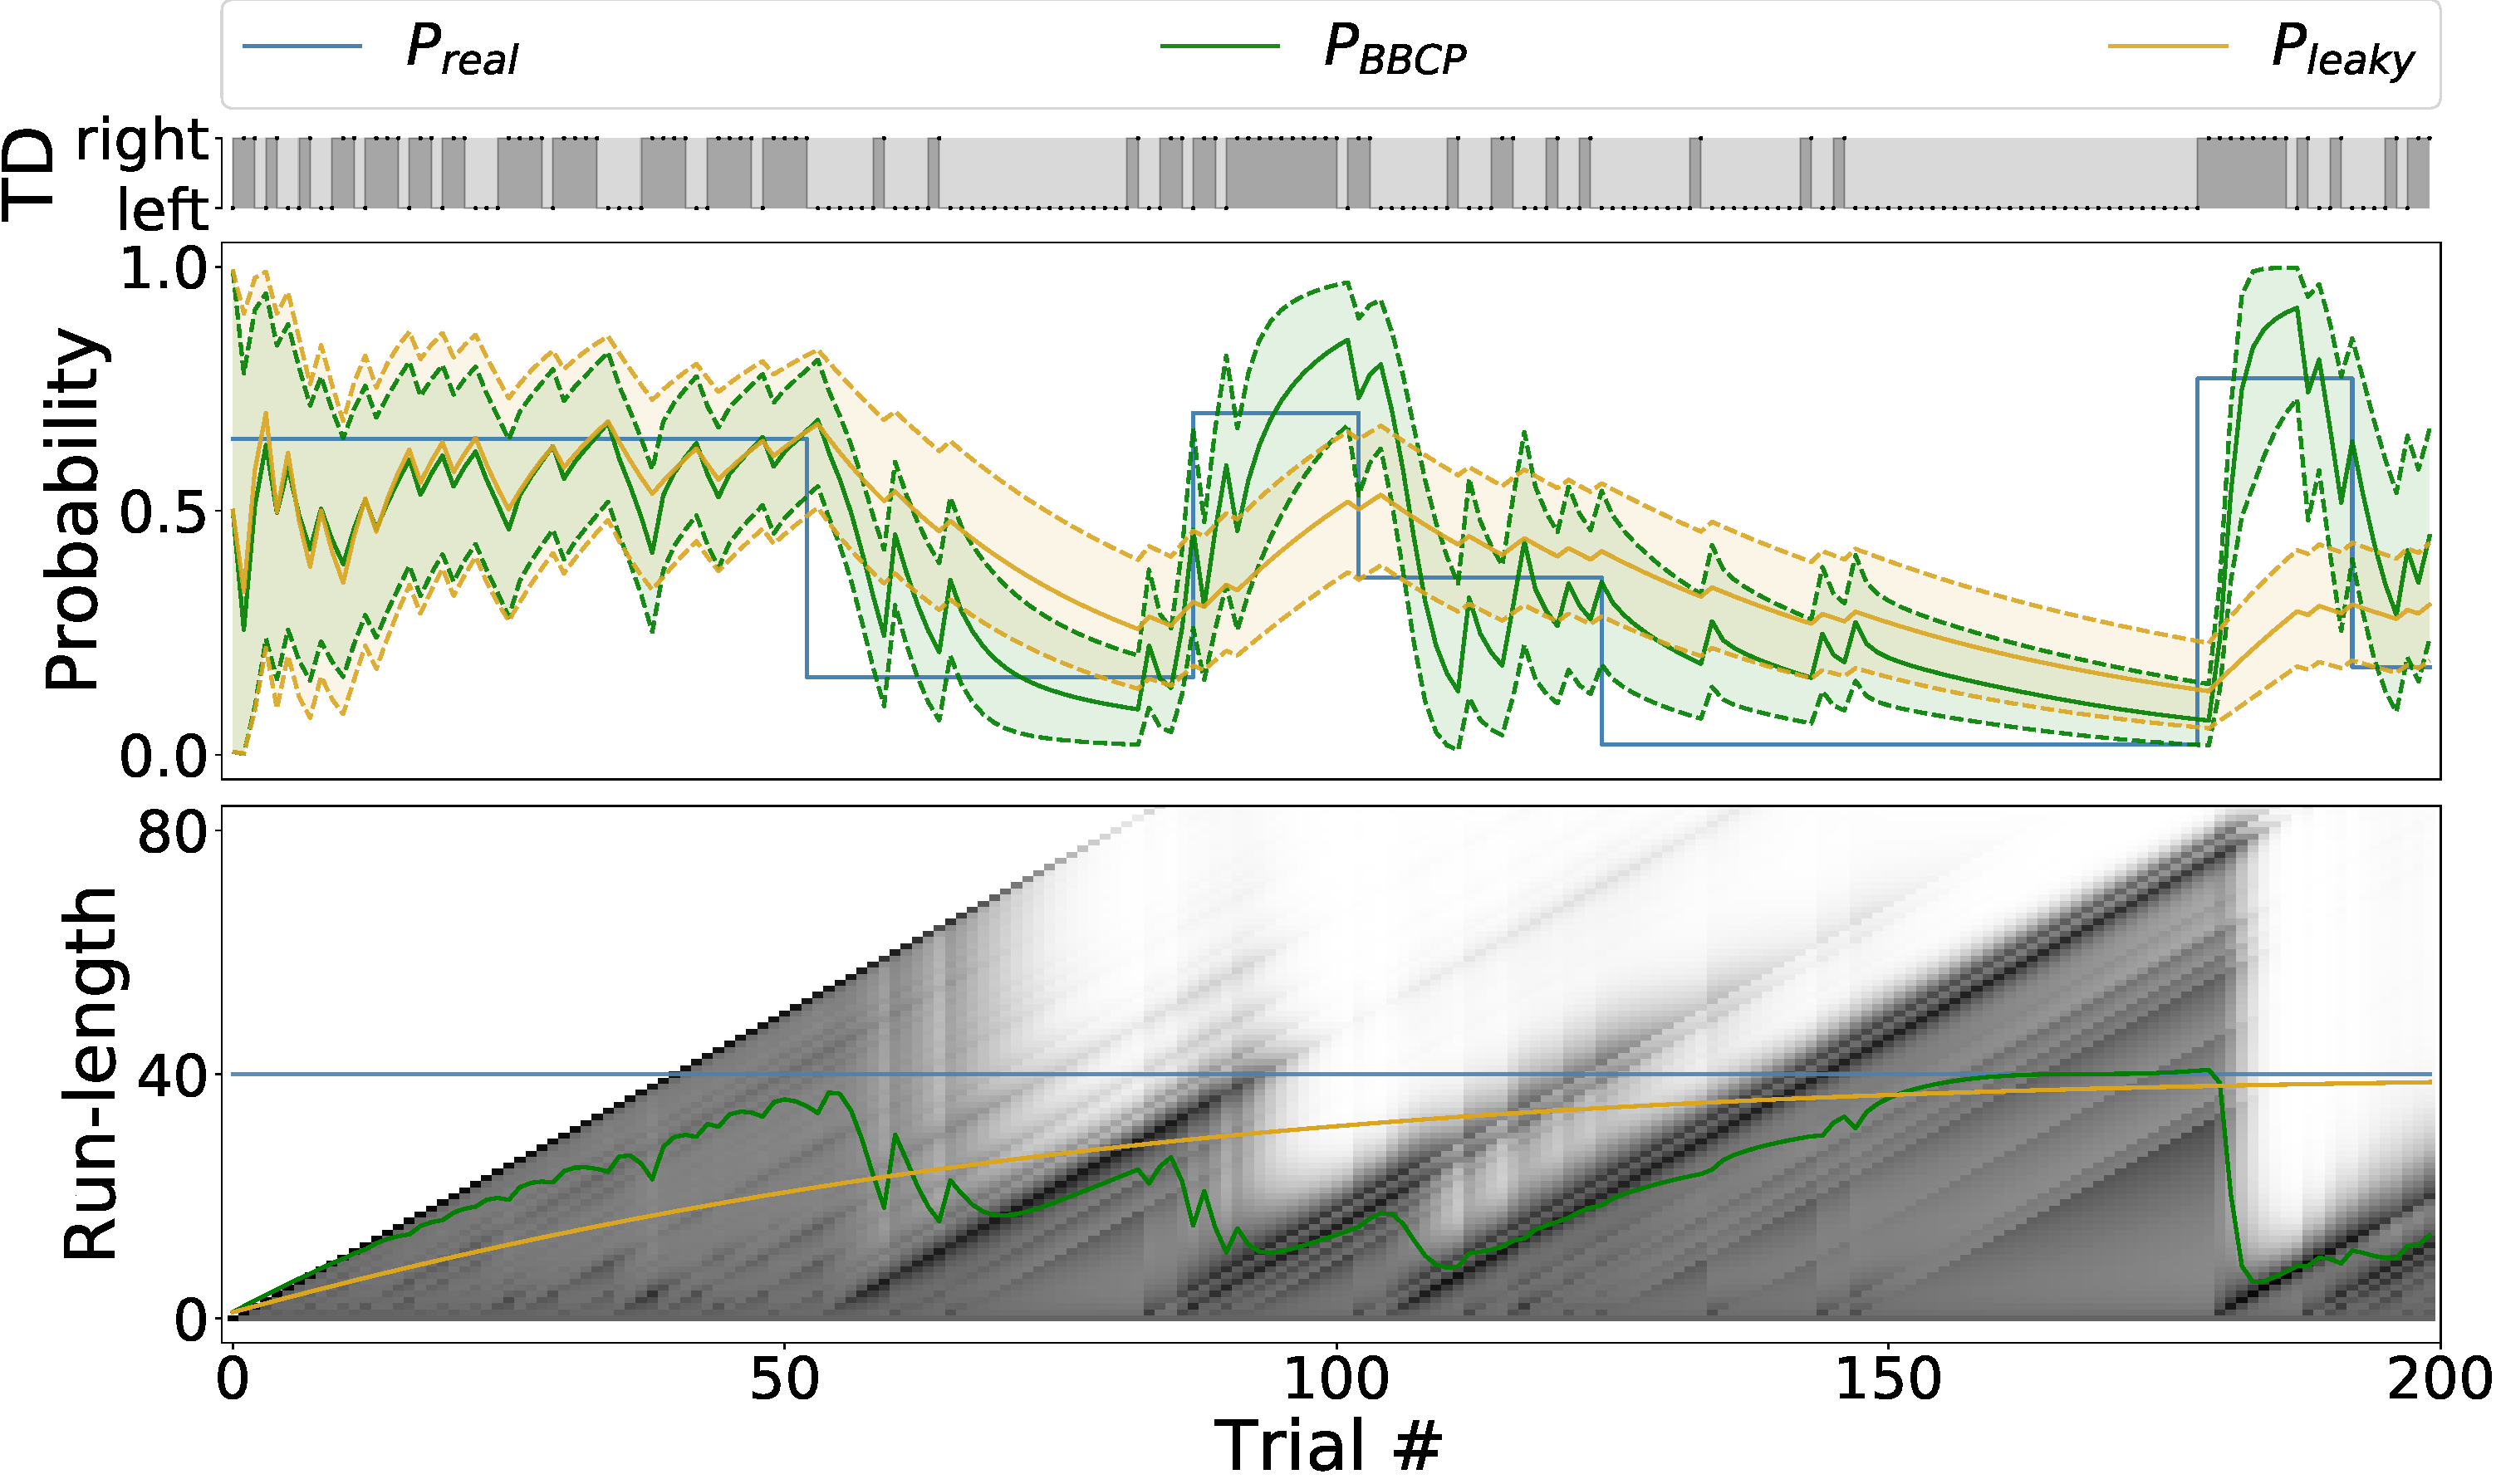
\includegraphics[width=0.618\linewidth]{3_BCP_readouts}};
\draw [anchor=north west] (0.000\linewidth, .62\linewidth) node {$\mathsf{(A)}$};
\draw [anchor=north west] (0.382\linewidth, .62\linewidth) node {$\mathsf{(B)}$};
\end{tikzpicture}
} 
\caption{\emph{Binomial Bayesian Change Point model (BBCP)}
~\textbf{(A)} This plot shows a synthesized sequence of $10$ events
that each correspond to a binomial choice, either $0$ or $1$,
which will then correspond to a leftward or rightward movement of the target (TD).
Here, the probability switched from a value of $.1$ to $.9$ at trial $5$.
The BBCP model tries to capture the occurrences of a switch by inferring run lengths,
that is, the number of trials since a switch.
At any new datum (trial), this defines a Hidden Markov Model
as a graph (treillis) of possible run lengths.
Edges of this graph indicate that a message is being passed
to update each node's probability.
Black lines denote a progression of the run length at the next step (no switch),
while red lines stand for the possibility that a switch happened:
The run length falls back to zero.
The black and blue curve respectively represent for
the actual and inferred run length of the simulated data
as a function of trial number.
~\textbf{(B)} On a longer sequence of $200$ trials,
characteristic of our psychophysical experiments (see~\seeFig{intro}-A), % and~\seeFig{results_raw}),
we show in the top plot
the actual events which are observed by the agent (TD, fine black lines),
along with the hidden dynamics of the probability bias $x_1$,
the value inferred by a leaky integrator ($\bar{x_1}^t$, green line)
and the results of the BBCP model 
in estimating the probability bias $\hat{x_1}^t$ (blue line),
along with $95\%$ confidence intervals (CI).
This shows that for the BBCP model,
the accuracy of the estimated value of the probability bias
is closer than that from the leaky integrator.
We show below the belief for the different possible of run lengths
as a function of the trial number. 
Darker colors denote higher probability. 
The blue line corresponds to the mean run-length which is inferred:
Note that, while it takes some trials to detect a switch,
they are correctly identified (diagonal lines) and
as shown above, integration is thus faster than for the leaky integrator.
}
\label{fig:bayesianchangepoint}
\end{figure}
%-------------------------------------------------------------%
%-------------------------------------------------------------%
%: 2Ba precision in our belief of \hat{p}
%-------------------------------------------------------------%
There is a crucial difference between the simple agent presented above
which believes that changes occur at a constant rate ($\hat{x_2}^t=h$, see~\seeEq{leaky2})
and one that would invert the binomial switching model (BSM, see~\seeEq{bsm}).
Indeed, at any trial during the experiment,
the agent may infer beliefs about the trajectory of the volatility $x_2^t$
which itself is driving the trajectory of the probability bias $x_1^t$.
Knowing that the latter is piece-wise constant,
an agent may therefore have a belief over the number of trials since the last switch.
This number, that we will call the \emph{run-length}, is useful in two manners.
First, it allows for the agent to restrict the estimation $\hat{x_1}^{t}$ of $x_1^t$
to only those samples $x_0^t$ produced since the last switch and until $t$.
Indeed, the samples $x_0^t$ occurred before the switch are drawn independently from the present true value $x_1^t$
and thus cannot help estimating the latter.
Second, it is known that for this estimate, the precision
(that is, the inverse of its variance)
grows linearly with the number of samples:
The longer the run-length, the sharper the corresponding (probabilistic) belief.
We have designed an agent inverting the BSM by extending
the Bayesian Change-Point (BCP) detection model~\citep{AdamsMackay2007}.
The latter model defines the agent as an inversion of a switching generative model
for which the observed data (input) is Gaussian.
We will here present an exact solution for the case of the BSM,
that is, where the input is binomial (see~\seeEq{bsm}).

%-------------------------------------------------------------%
%: 2Bb overcoming this difficulty using a latent variable - prediction/update cycle
%-------------------------------------------------------------%
In order to define in all generality the switch detection model,
we will describe the fundamental steps of its computation,
while giving the full algorithmic details in~\seeApp{bcp}.
In general, the goal of predictive processing
is to infer the probability $Pr(x_0^t | x_0^{0:t-1})$ of the next datum
knowing what has been observed and
the prior of the agent on the generation of the data.
To derive a Bayesian predictive model, we first introduce
the run-length as a latent variable which helps the agent to represent the input.
Knowing that the data is generated by the BSM (see~\seeEq{bsm}),
the run-length is either null at the moment of a switch,
or this length (in number of trials) is incremented by $1$ if no switch occurred:
\eql{\choice{
r^t = 0 \quad \text{if} \quad x_2^t=1 \\
\text{and else} \quad r^t = r^{t-1} +1 }\label{eq:run_length}}%see~\seeEq{run_length}
This may be represented in a graph
in which information will be represented at the different nodes for each trial $t$ (see \seeFig{bayesianchangepoint}-A).
Using this latent variable at each trial $t$ to represent our belief,
we will define the run length $r^t$ distribution
for all different hypotheses
and assign a probability strength at each node
as $\beta^{(r)}_t=Pr(r^t | x_0^{0:t-1})$
which allows to compute the marginal predictive distribution:
\eql{
Pr(x_0^t | x_0^{0:t-1}) = \sum_{r^{t}} Pr(x_0^t | r^{t}, x_0^{0:t-1}) \cdot  \beta^{(r)}_t
\label{eq:pred}
}

Using these definitions, we will define the BBCP
as an update / prediction cycle.
First, we will \emph{update} beliefs on all nodes
by computing the likelihood of the new datum $x_0^t$ 
knowing the current belief at each node
that we define as $\pi^{(r)}_t=Pr(x_0^t | r^{t-1}, x_0^{0:t-1})$.
Second, knowing this probability strength, % an estimate for our belief on the different variables at the previous trial $t-1$,
we can make a \emph{prediction} for our belief of the state at the current trial $t$,
prior to the observation of a new datum $x_0^{t+1}$.
Using a knowledge of $\beta^{(r)}_{t-1}$ at trial $t-1$ and
using the transition probabilities defined by~\seeEq{run_length},
this allows to predict the beliefs at each node:
\eqa{
\beta^{(r)}_t \propto \sum_{r^{t-1}}  Pr(r^t | r^{t-1}) \cdot  Pr(x_0^t | r^{t-1}, x_0^{0:t-1}) \cdot  \beta^{(r)}_{t-1}
\label{eq:pred_node}
}
where $\beta^{(r)}_t$ is scaled such that $\sum_r \beta^{(r)}_t = 1$.
In the graph, this corresponds to a message passing from the nodes at time $t-1$
to that at time $t$ and formalized by the transition matrix $Pr(r^t | r^{t-1})$.
Finally, this update / prediction cycle applied to the BSM and using~\seeEq{bsm}
will constitute the Binomial Bayesian Change Point (BBCP) detection model.

%-------------------------------------------------------------%
%: 2Bc online estimation: initialization
%-------------------------------------------------------------%
The main difference between our algorithm and that of~\citep{AdamsMackay2007},
is that the observed data is binomial and not Gaussian as in their case.
The random variable $x_1^t$ is the probability bias used
to generate the sequence of events $x_0^t$ through a binomial trial.
Mathematically, a belief on the probability bias $p$ defining the binomial trial (and thus to the process corresponding to the trial sequence),
is well represented by the conjugate probability distribution of the binomial distribution,
that is, by the beta-distribution $B(p; \mu, \nu)$.
It is parameterized here by its sufficient statistics,
the mean $\mu$ and sample size $\nu$
(see~\seeApp{likelihood} for our choice of parameterization).
First, beliefs are set at $t=0$ to prior values before observing the first trial.
In terms of probabilities, this amounts to set :
\eqa{
& \beta^{(0)}_0=Pr(r^0=0)=1 \text{,}\quad \forall r^0>0 \text{, } \beta^{(r)}_0=Pr(r^0)=0 \quad \text{and} \\
& Pr(x_1^0 | r^0=0) \propto B(x_1^0; \mu_{prior}, \nu_{prior})
}
where $\mu_{prior}$ and $\nu_{prior}$ represent the sufficient statistics
of the prior (Beta-distribution) probability density function (pdf) $\Pp$
for the probability bias
at the occurrence of a switch (in particular, at node $r^0=0$).
By recurrence, one can show that at any trial $t$,
this pdf will always be a beta-distribution,
and with sufficient statistics $(\mu^{(r)}_{t}, \nu^{(r)}_{t})$.
In the following, we will define the probability distribution at each node $r^t$,
knowing the data observed from the first trial and before $t$ such that
$
\pi^{(r)}_t = B( x_0^t |  \mu^{(r)}_{t}, \nu^{(r)}_{t})
$. %}
We can now detail the update / prediction cycle.

%-------------------------------------------------------------%
%: 2Bd update = Computing the likelihood
%-------------------------------------------------------------%
In particular, as we sequentially observe new data,
we will first implement an update step that
computes the likelihood of this datum $x_0^t$ with respect to
the current beliefs at trial $t$ at each node $r$.
In all generality, to perform this computation for some data $o$,
we have computed the probability of each model
parameterized by the mean $p$ and the sample size $r$
for the two hypothesis $o=1$ or $o=0$.
This defines the likelihood
$\Ll(o | p, r) = \frac{1}{Z} Pr(o |p, r)$
with $Z$ such that $\Ll(p | o=1, r) + \Ll(p | o=1, r)=1$.
It measures the relative frequency of observing an occurrence of $o$ at trial $t$,
as the updated estimation of the probability bias of $\frac{p\cdot r + o}{r+1}$
knowing a sample size of $r+1$.
Following the formulation of the Beta probability distribution, it follows:
\eql{% TODO: check formula
\Ll(o | p, r) = \frac{1}{Z} \cdot {(p\cdot r + o)}^{p\cdot r + o} \cdot {((1- p)\cdot r + 1- o)}^{(1- p)\cdot r + 1- o}
\label{eq:likelihood}
}
where
\eq{
Z = {(p\cdot r + 1)}^{p\cdot r + 1}  \cdot {((1- p)\cdot r )}^{(1- p)\cdot r }  +
    {(p\cdot r )}^{p\cdot r }  \cdot {((1- p)\cdot r + 1)}^{(1- p)\cdot r + 1}
}
The derivation of this function is detailed in~\seeApp{likelihood}.

%-------------------------------------------------------------%
%: 2Be online estimation: prediction
%-------------------------------------------------------------%
In the second step, one can perform prediction
using the graph defined in \seeFig{bayesianchangepoint}-A.
Now that we have the vector of likelihoods $\pi^{(r)}_t=\Ll(x_0^t |  \mu^{(r)}_{t}, \nu^{(r)}_{t})$,
one can update probabilities and perform the next prediction for trial $t+1$.
The transition matrix % defined by the graph,
allows to compute growth probabilities for each run-length $r \geq 0$, 
that is, the belief at the next trial before observing a new datum:
\eqa{
\beta^{(r+1)}_t = \frac{1}{B} \cdot \beta^{(r)}_{t-1} \cdot \pi^{(r)}_{t} \cdot (1-h)
}
(where $h$ is the scalar defining the hazard rate)
but also the change-point probabilities:
\eqa{
\beta^{(0)}_t  = \frac{1}{B} \cdot \sum_{r} \beta^{(r)}_{t-1} \cdot \pi^{(r)}_{t} \cdot h
}
with $B$ such that $\sum_{r} \beta^{(r)}_{t} = 1$.
On the other hand, we update the sufficient statistics to be used 
in the computation of the likelihood at the next trial following:
\eqa{
& \mu^{(0)}_{t+1} = \mu_{prior} \text{,} \quad \nu^{(0)}_{t+1} = \nu_{prior} \\
& \mu^{(r+1)}_{t+1} = r/(r+1) \cdot \mu^{(r)}_{t} + 1/(r+1) \cdot x_0^t \text{,} \quad \nu^{(r+1)}_{t+1} = \nu^{(r)}_{t} + 1
}
Note that $\mu^{(r+1)}_{t+1}$ is a moving average at trial $t$ on the $r$ last samples,
and $\forall r, t; \nu^{(r)}_{t}$ is the sample size corrected by the initial condition:
$\nu^{(r)}_{t} = r + \nu_{prior}$.
This updates for each node the sufficient statistics of the pdf at the current trial.
This finalizes the prediction step.

The agent may infer at each trial the belief
and use for instance the expected value or the maximum a posteriori as readouts.
More precisely, we define these two strategies as following:
Either by choosing
at each trial the run-length with maximal probability
and then assigning the predicted probability bias
as the probability bias for that run-length:
\eql{
\hat{x_1}^t = \mu^{(r^\ast)}_{t} \quad \text{with} \quad r^\ast = \argmax_r \beta^{(r)}_{t}
}
A second strategy consists in computing
at each trial the conditional mean of the probability bias
as the expected value over all run-lengths:
\eql{
\hat{x_1}^t = \sum_{r} \beta^{(r)}_{t} \cdot \mu^{(r)}_{t}
}
Contrary to the leaky integrator for which the inference $\hat{x_2}=h$ was fixed,
the BBCP model uses a dynamical model, but still with only one parameter.
As for the latter, this parameter~$h=\frac 1 \tau$ informs the BBCP model
that the probability bias  changes \emph{on average} every~$\tau$ trials.
As in \seeEq{leaky}, this defines the \emph{hazard rate}.
Note that the resulting operations are online, that is,
that only the belief at trial $t$ and the new datum $x_0^t$
are sufficient to predict all probabilities.
%at the next trial $t+1$: $Pr(r_t | x_0^{0:t})$, $\mu^{(r)}_{t+1}$ and $\nu^{(r)}_{t+1}$.
%projecting beliefs backwards and forward  : the algorithm is online et the price of memory
% ------------------------------------------------------------------
\subsection{Quantitative analysis of the Bayesian change point algorithm}
% ------------------------------------------------------------------
%-------------------------------------------------------------%
%: 2Ca python scripts : qualitative analysis
%-------------------------------------------------------------%
This algorithm is detailed in~\seeApp{bcp} and 
we have implemented it using a set of python scripts.
This implementation provides also with some control scripts
to test the behavior of the algorithm with synthetic data.
Indeed, this allows to qualitatively and quantitatively asses
this ideal observer with a known ground truth before applying it
on the trial sequence that was used for the experiments and 
ultimately comparing it to the human behavior. % (see~\seeFig{results_raw}).
%TODO : synchronize with FIGURE 3 fig:bayesianchangepoint
\seeFig{bayesianchangepoint}~\textbf{A} shows for illustration purpose
one instance of a short sequence of simulated data $x_0^t$
of leftward and rightward trials with a probability $x_1^t$
of being rightward with possible variations across time.
It also shows the predicted probability $\hat{x_1^t}$
as computed using the BBCP algorithm.
It illustrates
the belief on the predicted probability $\hat{p}$ at a given trial.
On \seeFig{bayesianchangepoint}~\textbf{B},
we applied the BBCP model to 
a longer sequence of $200$ trials,
characteristic of our psychophysical experiments.
Below, 
we can see the dynamical evolution of the belief on the latent variable (run length),
while we show above the results of the inference along with confidence intervals.
As for the synthetic example above,
there is a correct detection of switch after a short delay of a few trials,
as shown with the comparison with the ground truth.
We remark two main observations.
First, after each detected switch, beliefs align along a linear ridge,
as our model integrates belief about a current phase during two switches (it 'stays').
Then, we observe that after a switch (hidden to the model),
the belief is diffused strongly until the relative probability
is less that that assigned to a lower run-length:
There is a transition to a new state (it 'goes').
Second, we may use this information to read-out the most probable probability-bias and the confidence interval
as shown by the red dashed lines (respectively $.05$ and $.95$).
Note, the fixed-length is simply implemented
by an agent with a fixed run-length $r_t=\tau$ (see broken dashed line in \seeFig{bayesianchangepoint}~\textbf{B})
this allows for a simple comparison of the BBCP model with the leaky integrator.
Again, we see that a fixed length model gives a similar output
but with the two disadvantages described above, namely that
1/ the delay after the occurrence of a switch will always be similar,
2/ there is no dynamic update of the inferred probability 
while in the BBCP model, the precision of each new datum 
is higher after a switch.
In particular, from this correct detection,
the value of the inferred probability converges more rapidly to the ground truth
as the number of observations increase after a switch.

%-------------------------------------------------------------%
%: 2Cb quantitative analysis / different read-outs
% see 2018-02-12 journal club bayesian changepoint chloe.pdf p.33/ p.42
% TODO include these quantitative results in a figure
%-------------------------------------------------------------%
Let's now see the application of our model when applied
to the experimental protocol
that we used in our psycho-physical experiments.
To quantitatively evaluate the algorithm,
we computed the  negative log-likelihood (in bits) of the estimate
knowing the ground truth 
and averaged over all trials:
\eql{
\Cc =  \sum_{t} -\log_2 B(x_1^t ; \hat{x_1}^t, r^t )
}
This measure explictly corresponds to the average score of our model,
where the score is the likelihood of the inferred belief about the probability bias
as given by its mean $\hat{x_1}^t$ along with its precision $r^t$ and
compared to the hidden ground truth $x_1^t$. 
%\eql{
%B(x_1^t ; \hat{x_1}^t, r^t ) =  \sum_{t} -\log_2 B(\hat{x_1}^t ; x_1^t, r^t )
%}
Similar measures based on the predicted readout $\hat{x_0}^t$
gave similar results but would need more data to converge.
We have tested $100$ blocks of $2000$ trials for each read-out.
In general, we found that the inference is better for the 'mean' read-out
than for the 'max' read-out and lowest for the 'fixed' read-out.
Moreover, by testing different values of $h$ assumed by the agent
but for a fixed $h=1/40$ in the BSM,
we found that this is true for a range of values of $h$.
Importantly, this shows that inference is best for a hazard rate
equal to that in the generative model and which is hidden to the model.
This property will be important to guess the hazard rate assumed by an individual agent
when we observe the set of responses it gives to a given sequence of stimuli
(see~\seeSec{inter}).

%-------------------------------------------------------------%
%: 2Cc perspectives
%-------------------------------------------------------------%
There are limits to the agent that we have defined.
First, data is considered to be a sequence of discrete steps.
A similar approach using a Poisson point process 
allows to extend to the continuous time
such as in the framework of~\citet{RadilloBrady2017}:
In this experiments, authors analyzed the licking behavior of rats in a dynamic environment.
This extension is beyond the scope of our current protocol,
but could consist in a natural extension of the protocol
to more complex and ecological settings about the timing of stimuli.
Then, remember that the only free parameter of this model is the hazard rate $h$
assumed by the agent (as in the fixed-length agent).
Though there exist more generic solutions~\citep{Wilson13,Wilson18},
we will keep this parameter fixed for any fitted agent, but evaluate
how well it fits to the experimental outcomes at the different scales of the protocol:
within sub-blocks, for each sub-block or for any individual observer.
As a summary, for any given sequence,
we get an estimate of the probability bias assumed by the ideal observer.
We will now see how we can apply that to our experimental protocol.
In particular, we expect intuitively the results to be more variable
compared to the previous protocol with fixed-length blocks (see~\seeFig{intro}-C).
%: %%%%%%%%%%%%%%%%%%%%%%%%%%%%%%%%%%%%%%%%%%%%%%%%%%%%%%%%%%%%%%%
%\section{Results: psychophysics}
%%%%%%%%%%%%%%%%%%%%%%%%%%%%%%%%%%%%%%%%%%%%%%%%%%%%%%%%%%%%%%%
%%%%%%%%%%%%%%%%%%%%%%%%%%%%%%%%%%%%%%%%%%%%%%%%%%%%%%%%%%%%%%%
\section{Results: Eye movements recordings}
%%%%%%%%%%%%%%%%%%%%%%%%%%%%%%%%%%%%%%%%%%%%%%%%%%%%%%%%%%%%%%%
\label{sec:results_psycho}
%: FIGURE 2 fig:results_psycho ~\seeFig{results_psycho} 
\begin{figure}%[b!]
\centering{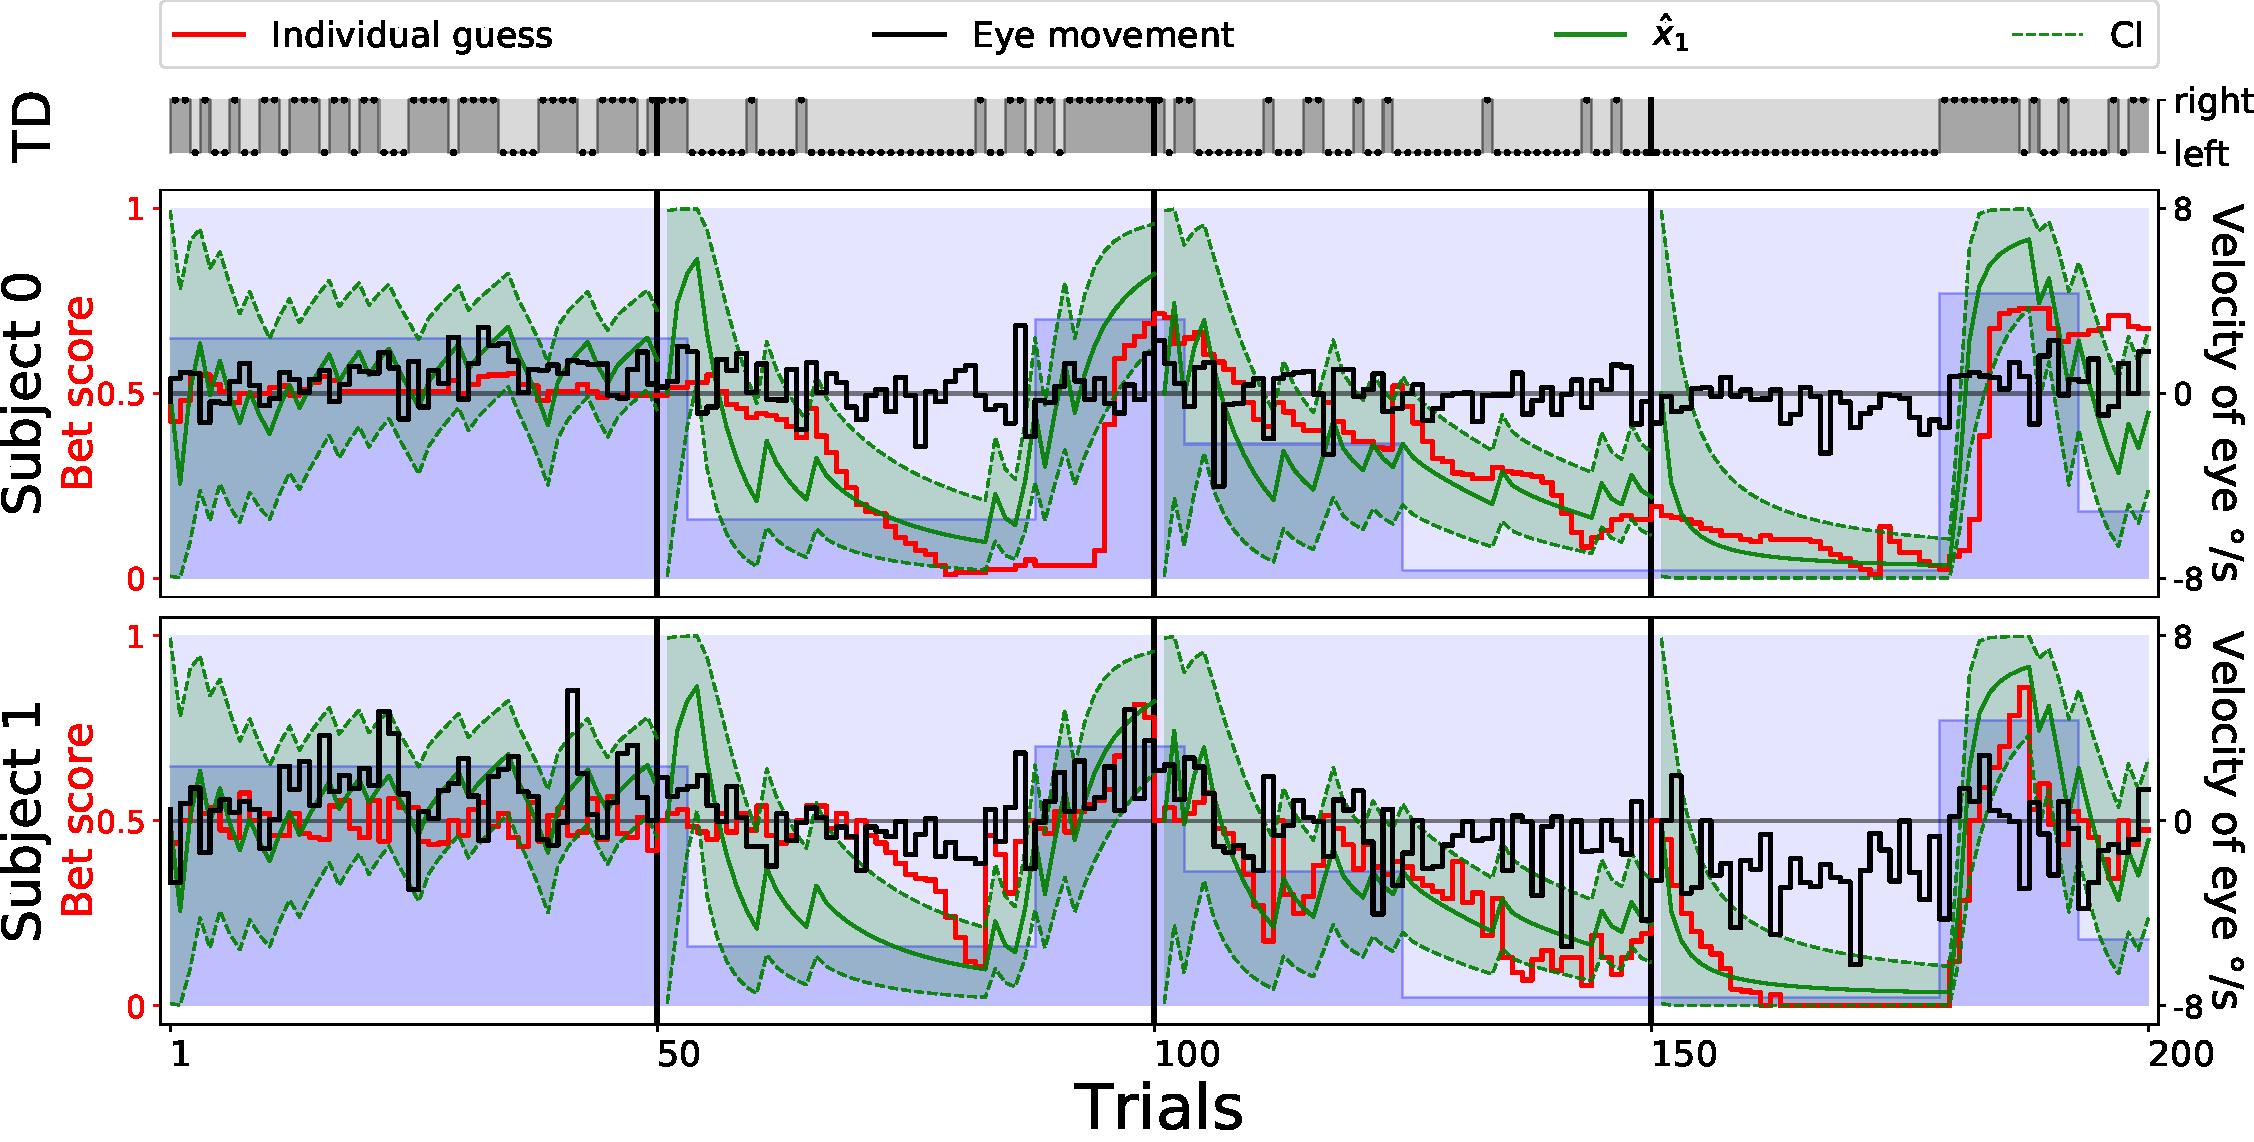
\includegraphics[width=\linewidth]{2_results_enregistrement}}
\caption{
\emph{Behavioral results.} %
The top row represents the sequence of target directions (TD)
that were presented to observers
for a sequence of $200$ trials
as generated by the binomial switching model (see~\seeFig{intro}-A).
Bottom rows show the raw behavioral results 
for two representative observers:
The recorded aSPEM strength as measured 
by the horizontal eye velocity estimated right before
the onset of the visually-driven SPEM (black line);
and the bet score as given by the rating scale (red line).
These values were here scaled according to their extremal values.
We also show the evolution of the value 
of the probability bias $p$ (red shaded areas)
which is hidden to observers
and used to generate the TD sequence.
We have overlaid the results of the BBCP model 
(see~\seeFig{bayesianchangepoint}-B, blue line).
This shows qualitatively a good fit between 
the experimental evidence and the model. 
Note that we introduced short pauses 
every $50$ trials (as denoted by vertical black lines), 
to prevent from fatigue and check for possible drifts of the recorded eye position.
}
\label{fig:results_psycho}
\end{figure}
%-------------------------------------------------------------%
%-------------------------------------------------------------%
%: 3A raw results in aSPEM
%-------------------------------------------------------------%
We used the BSM model
to generate the (pseudo-)random sequence of
the dot's directions (the alternating output of leftward/rightward trials)
as the sequence of observations.
In a first session, we recorded the participants' eye movements and 
extracted the aSPEM velocity (for details, \seeApp{em}).
Among our $12$ subjects,
we show two representative examples in~\seeFig{results_psycho}.
These representative participants were chosen as that
with the median fit in the quantitative analysis
that will follow (\seeSec{inter}).
In particular, we show in the top panel the actual sequence of binary choices
(TD, leftward or rightward) of the Bernoulli trial  and 
in the bottom panels, we compare the evolution of the recorded aSPEM with
the ground truth value of the (hidden) probability bias $x_1$
and the value inferred using the BBCP model (see~\seeFig{bayesianchangepoint}-B,
as a blue line, along with its confidence interval in a shaded area).
Comparing the raw eye movement results with the latter,
it seems qualitatively that both traces evolve in good agreement.
First, one can observe in both a trend with the polarity of aSPEM velocity
to be negative for $p$ values below~$.5$ and positive for values above~$.5$.
Moreover, both curve seem to lag of few trials 
after the occurrence of a switch
(also hidden to the observers).
Both have similar delays in \emph{detecting} and taking into account a switch,
reflecting the time (in the order of a few trials) taken to integrate enough information
to switch to a novel probability bias value for the Bernoulli trial.
In general, results are more variable when the bias is weak ($p\approx .5$)
than when it is strong (close to zero or one),
consistent with the dependence of the variance of a Bernoulli trial
as a function of the probabilistic bias ($var(p)= p \cdot (1-p)$).
More precisely, the precision (i.e. the inverse of the variance)
of the inferred probability-bias $\hat{p}$ seems to increase
in bigger sub-blocks as information is integrated over more trials.
As a result, the inferred probability as a function of time
seems qualitatively to constitute a reliable regressor
for predicting the strength of aSPEM.

%: <----- Laurent is here ----->
%-------------------------------------------------------------%
%: 3B Results: bias rating scale measurements
%-------------------------------------------------------------%
\label{sec:rating_scale}
%: qualitative analysis \seeFig{results_psycho}-B
As we could assess qualitatively in~\seeFig{results_psycho},
the trace of the rating scale seems to correlate well
with the inferred probability $\hat{p}$.
%In addition, the explicit bet score
%for the next trial's motion direction
%seems to follow a similar trend.
Similarly to the strength of aSPEM, we actually found that:
(1) The series of the paricipants' bias guesses exhibits a positive correlation with $\hat{p}$:
as a consequence, the next outcome of $x_{0}^{t}$ will in general be correctly inferred,
as compared to a random choice. %\AM{DID WE ACTUALLY PERFORM THIS COMPARISON?} - LP  it is visual / we could do it / I do not know if that would be useful...
(2) A stronger bias leads to a lower variability in the bias estimate.
(3) A (hidden) switch in the value of the bias is
most of the time correctly identified after only a few trials.
Note also that at every pause (black vertical bar in~\seeFig{results_psycho}),
participants tended to favor unbiased guesses, close to $0.5$
than at the end of a sub-block of trials.
We can speculate that this phenomenon would correspond to a resetting mechanism of the internal belief on the probability bias.
As a consequence, the experiment performed in the second session
shows that the probability-bias values that are consciously estimated by participants
are qualitatively similar to the implicit (and unconscious) ones which supposedly underlie the generation of anticipatory aSPEM with variable strength.

%-------------------------------------------------------------%
%: FIGURE 4  fig:results_psycho \seeFig{results_psycho}
\begin{figure}%[b!]
\centering{
\begin{tikzpicture}%[thick,scale=1, every node/.style={scale=1} ]
\node [anchor=north west]  (img4) at (0.000\linewidth,.618\linewidth){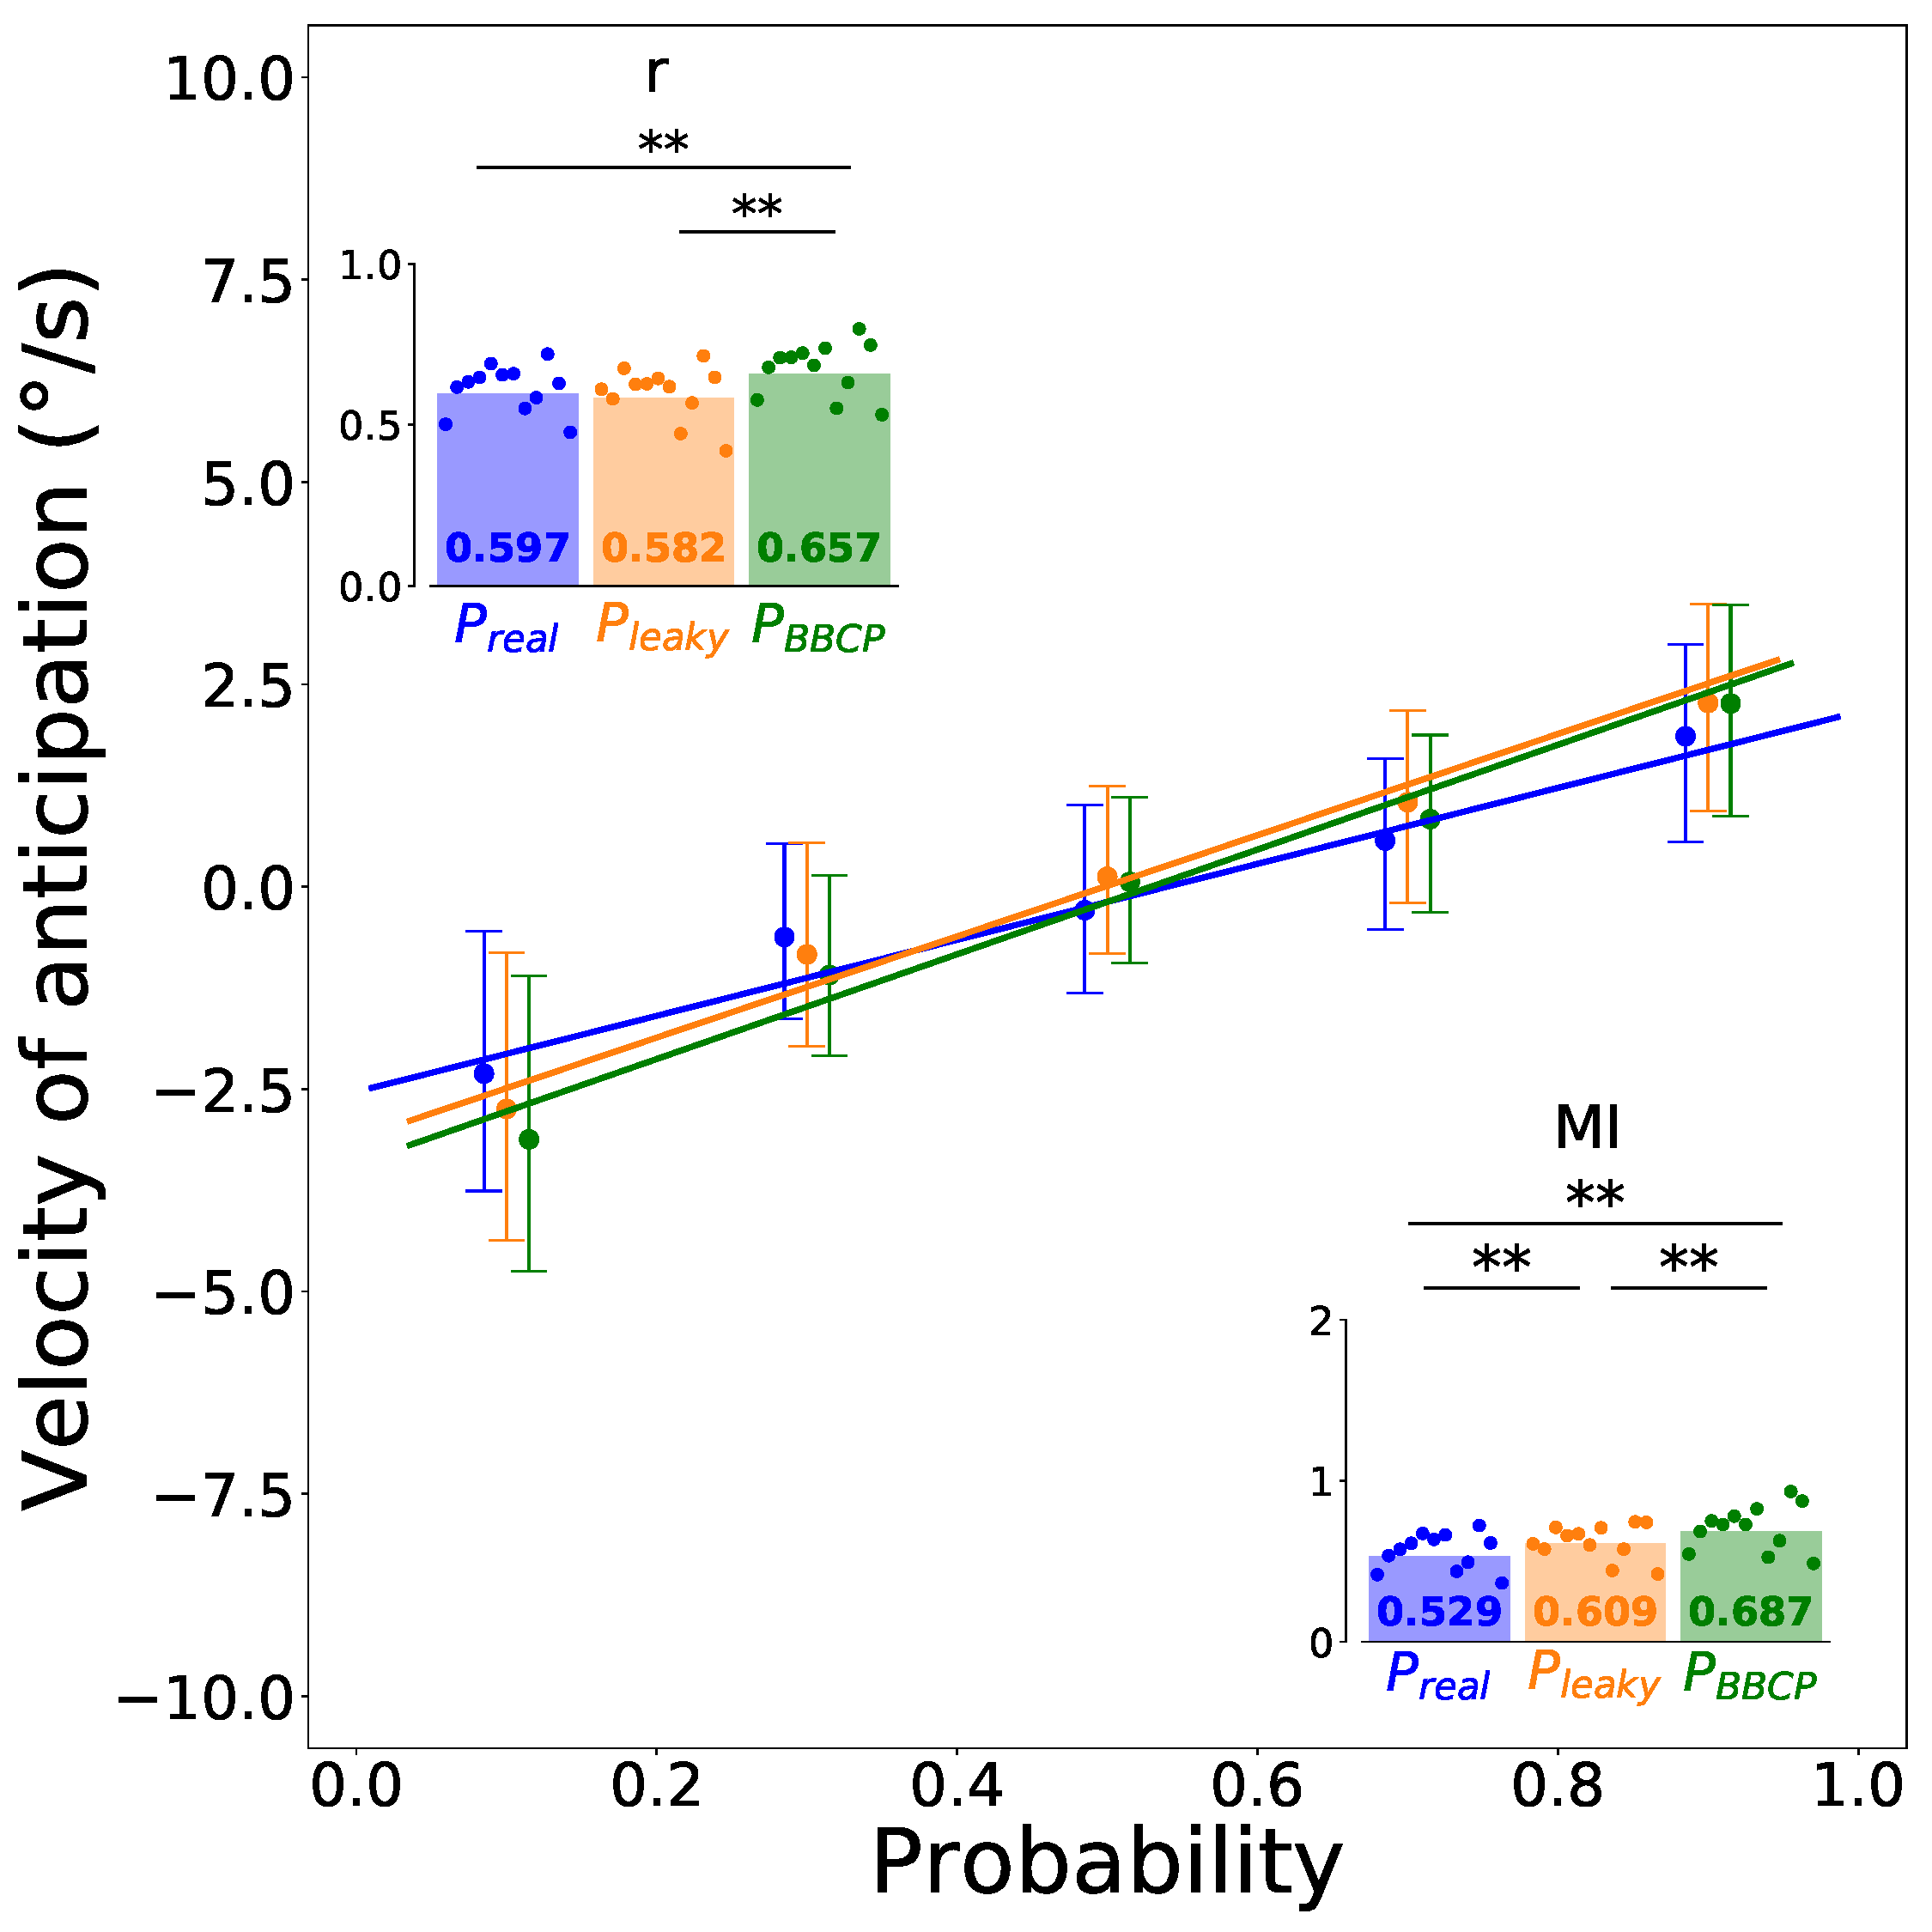
\includegraphics[width=0.49\linewidth]{4_A_result_psycho_aSPEM}};
\node [anchor=north west]  (img4) at (0.51\linewidth,.618\linewidth){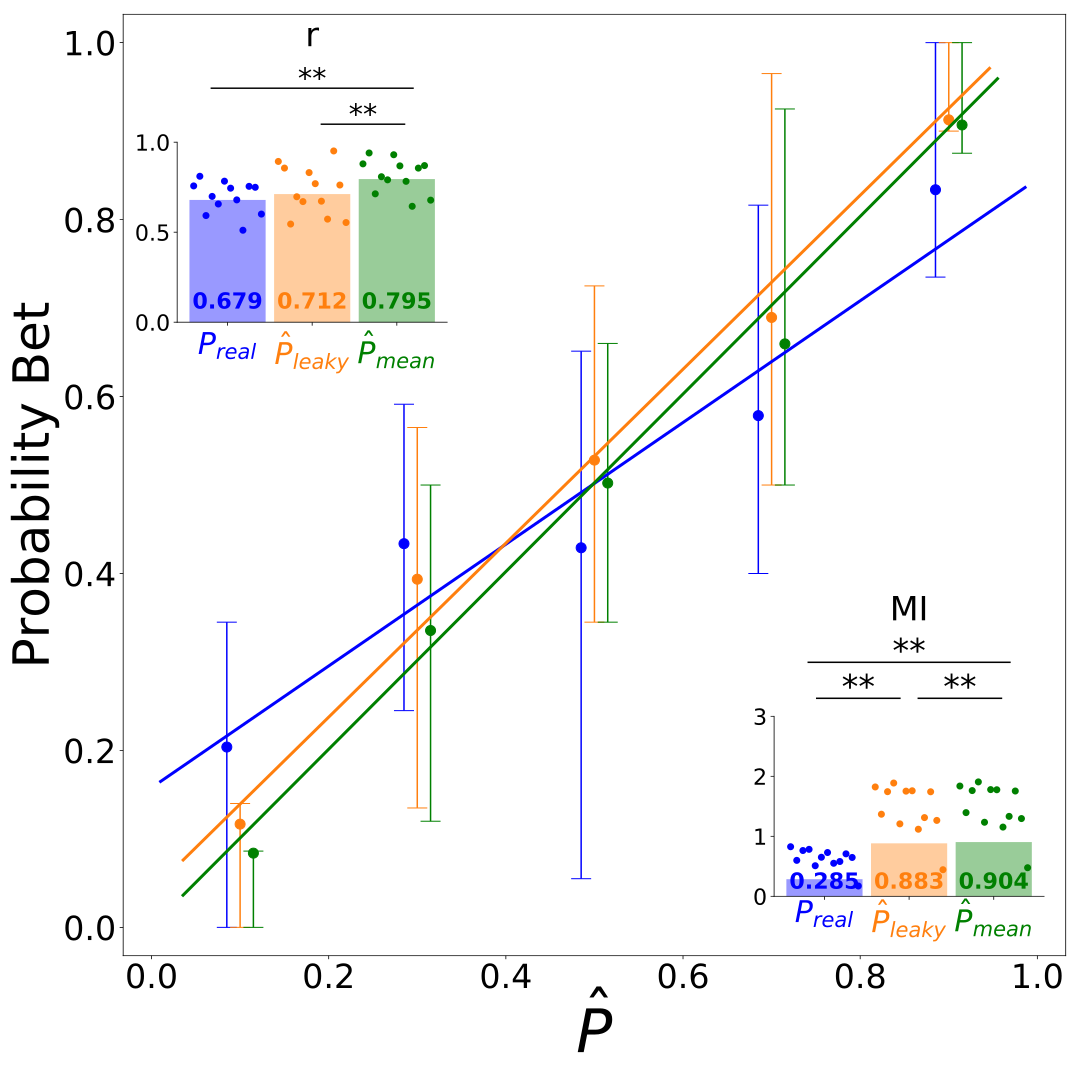
\includegraphics[width=0.49\linewidth]{4_B_result_psycho_bet}};
%
\draw [anchor=north west] (0.000\linewidth, .618\linewidth) node {$\mathsf{(A)}$};
\draw [anchor=north west] (0.5\linewidth, .618\linewidth) node {$\mathsf{(B)}$};
%
\end{tikzpicture}
}

\caption{ \emph{Psychophysical results over all participants}
%\CP{Attention KDE mean !}
Each trial in our experimental results in an estimate of
the strength of aSPEM (as measured by VEM)
and a rating scale value.
Relating those values with the corresponding inferred value $\hat{p}$
of the probability bias,
this constitutes a scatter of values.
We display these relationships using a
Kernel Density Estimation (KDE) of the relationship between $p$ (abscissa)
and \textbf{(A)} VEM and \textbf{(B)} the value of bet (in ordinates).
In \textbf{(A)}, we have overlaid is a regression line which shows
a high correlation factor ($R=XXX$) which is superior to that found
with the fixed-length design (see Appendix ...)
but also with other models described in the text
(fixed-length estimator, maximum BBCP - see Appendix ... ).
In \textbf{(B)}, we have fitted the data with a logistic regression
showing a negligeable intercept (no bias) linked to the symmetry
of the problem, but a consistent slope showing an aversion to risk
(cf Kahneman13).
%\textbf{(C)}
% we should comapre with the original slope obtained by Anna?
}
\label{fig:results_psycho}
\end{figure}
%%-------------------------------------------------------------%
%-------------------------------------------------------------%
%: 3C quantitative analysis
%-------------------------------------------------------------%
Similarly to~\seeFig{results_psycho}-A,
we now compare quantitatively the value of rating scale
as measured during the second experimental session with the model-inferred $\hat{p}$.
The KDE estimate shown in~\seeFig{results_psycho}-B,
represents the relationship between
the model-estimated probability-bias
and the rating value which was provided at each trial
by participants for the outcome of the next trial.
This analysis exhibits a consistent relationship
but which now follows a non-linear trace.
In particular, the fit was more accurate
in comparison with
the forgetful agent (see~\seeApp{results_psycho}).
We modeled this behavior as
a logistic regression over
the log-odd ratio estimated by the agent.
%TODO model this relationship by a logistic regression
This analysis provides with regression factors for each participant.
It shows that the bias (intercept)
was negligible, while the slope (logistic factor)
was always positive.
This indicates a generic aversion to risk~\citep{Kahneman13}
such that the value of a possible outcome
is down-weighted by the precision of the inference.
Our logistic regression analyses
suggests that this may come from a multiplicative weight
on the (log-) odd-ratio which is chosen as a rating scaled
compared to the (log-)odd-ratio of the inferred probability. %\AM{Is it worth to discuss more in depth the different functional dependence on p of the two experimental measures? Cite Santos and Kowler discussion about this!} - LP: that would certainly be a great addition...


%: quantitive analysis
Quantitatively, we wished to look at the quality of the fit
between the strength of aSPEM and
the probability $\hat{p}$ computed by the BBCP algorithm.
In~\seeFig{results_psycho}-A, we have plotted for all subjects
this strength as a function of the inferred probability
that was coded at the second layer and which is unknown to the observer.
% TODO: First, the trend that we put in evidence is the identity of the observer
As we can see in~\seeFig{results_psycho}-A,
the probability $\hat{p}$ computed by the BBCP algorithm
is positively linearly correlated with the aSPEM velocity.
The corresponding Pearson correlation coefficient
is slightly higher than that found in
the classical experiment with fixed blocks~\seeFig{intro}-B.
Note that since the BBCP is a probabilistic model,
we can also compute the Mutual Information and
compare that value with that obtained by other models.
This analysis is presented in~\seeApp{bcp}).
This relatively strong correlation is surprising at a first sight as the probability blocks have random length,
and participants have to adapt to such a volatile environment.
However, when faced with some new observations,
the observer has to constantly adapt his response
to either exploit this information by considering that
this observation belongs to the same sub-block or to explore
a novel hypothesis.
This compromise is one of the crucial component that we wish to explore
and which is well captured by the BBCP model.
In particular, the model predicts the different facets
from the experimental results,
from the variability as a function of the inferred probability,
to the dynamics of the bahavior following a (hidden) switch.
As a consequence this leads to a stronger correlation,
as measured by the Pearson coefficient and Mutual information.
We deduce that the trace of inferred probabilities is a powerful regressor
to explain the strength of aSPEM.
We will now try to extend this result
to the second experimental session
where participants had to provide their rating scales.

%%%%%%%%%%%%%%%%%%%%%%%%%%%%%%%%%%%%%%%%%%%%%%%
\section{Results: Analyzing inter-individual differences}
%%%%%%%%%%%%%%%%%%%%%%%%%%%%%%%%%%%%%%%%%%%%%%%
\label{sec:inter}
%: separate above analysis
So far, our quantitative analysis was performed independently
for the different participants.
In particular, we have shown a representative example in~\seeFig{results_psycho}
but results varied across participants (see~\seeApp{results_psycho}).
This was best characterized qualitatively in both sessions by differences
in the variability of the responses but also for instance
with different characteristic delays after a switch.
This reflects the spectrum of individual choices
between the behaviors of exploration versus exploration ~\citep{Behrens07}.
Here, we were interested in characterizing the preference
of each individual participant, but also to characterize
if this preference covaried across the two sessions.
Crucially, we have seen that the BBCP model is controlled by a single parameter,
the hazard rate, or equivalently by its inverse, the characteristic time $\tau$.
Also, we have shown that knowing an observed sequence of behavioral responses,
we could fit the best value of $\tau$ which would explain it~\seeFig{bayesianchangepoint}-C.
Thus, by extracting the parameters for every subject
we can expect to characterise inter individual differences.

%: results
%-------------------------------------------------------------%
%: FIGURE 5  fig:results_inter \seeFig{results_inter}
% TODO présente une meta analyse qui montre une correlation par sujet (scatter plot) entre h_a et h_bet (see 2017-11-16 chloe figures.pdf ) y-a-til un continuum entre explorateurs et conservatezurs?, voir de montrer une causalité entre les 2 expériences - on pourrait superposer aussi les résultats si on avait utilisé un fixed-length ?
% cf https://github.com/laurentperrinet/bayesianchangepoint/blob/master/notebooks/test_hazardrate.ipynb
% cf : 4_Meta_analysis.ipynb
\begin{figure}%[b!]
\centering{
\begin{tikzpicture}%[thick,scale=1, every node/.style={scale=1} ]
%\node [anchor=north west]  (img4) at (0.000\linewidth,.588\linewidth){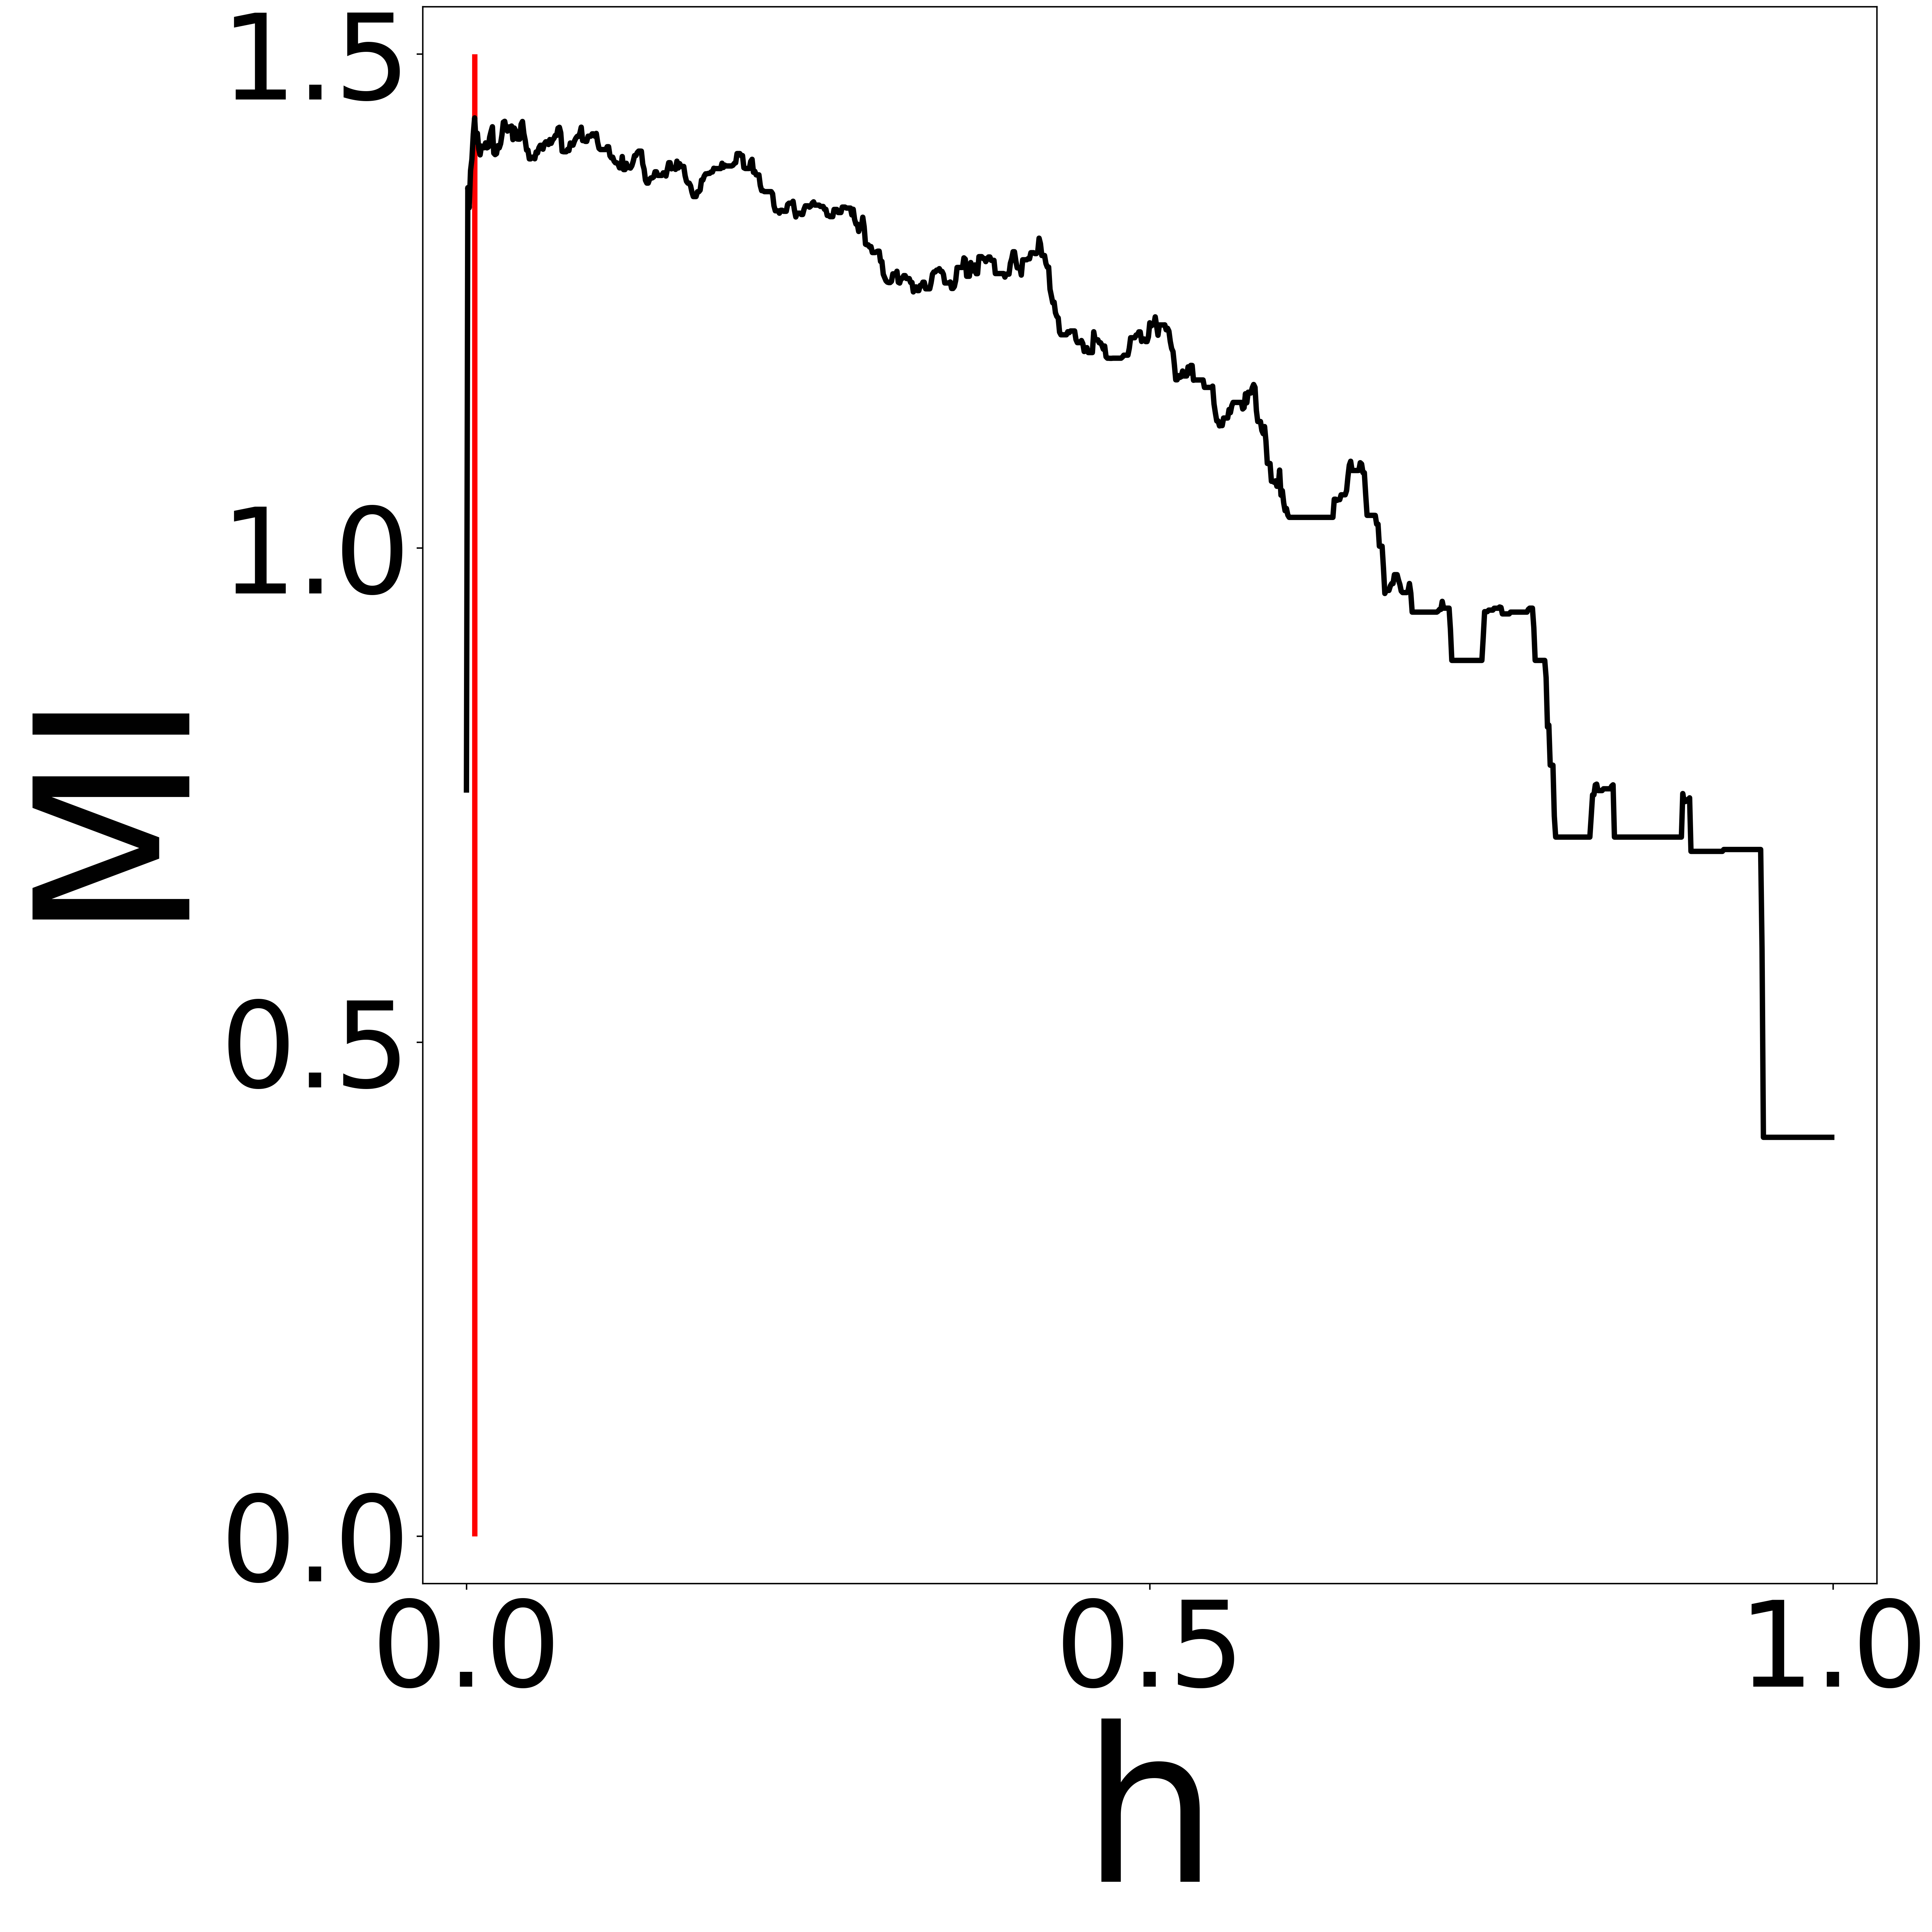
\includegraphics[width=0.25\linewidth]{5_A_h_bet}};
%\node [anchor=north west]  (img4) at (0.000\linewidth,.28\linewidth){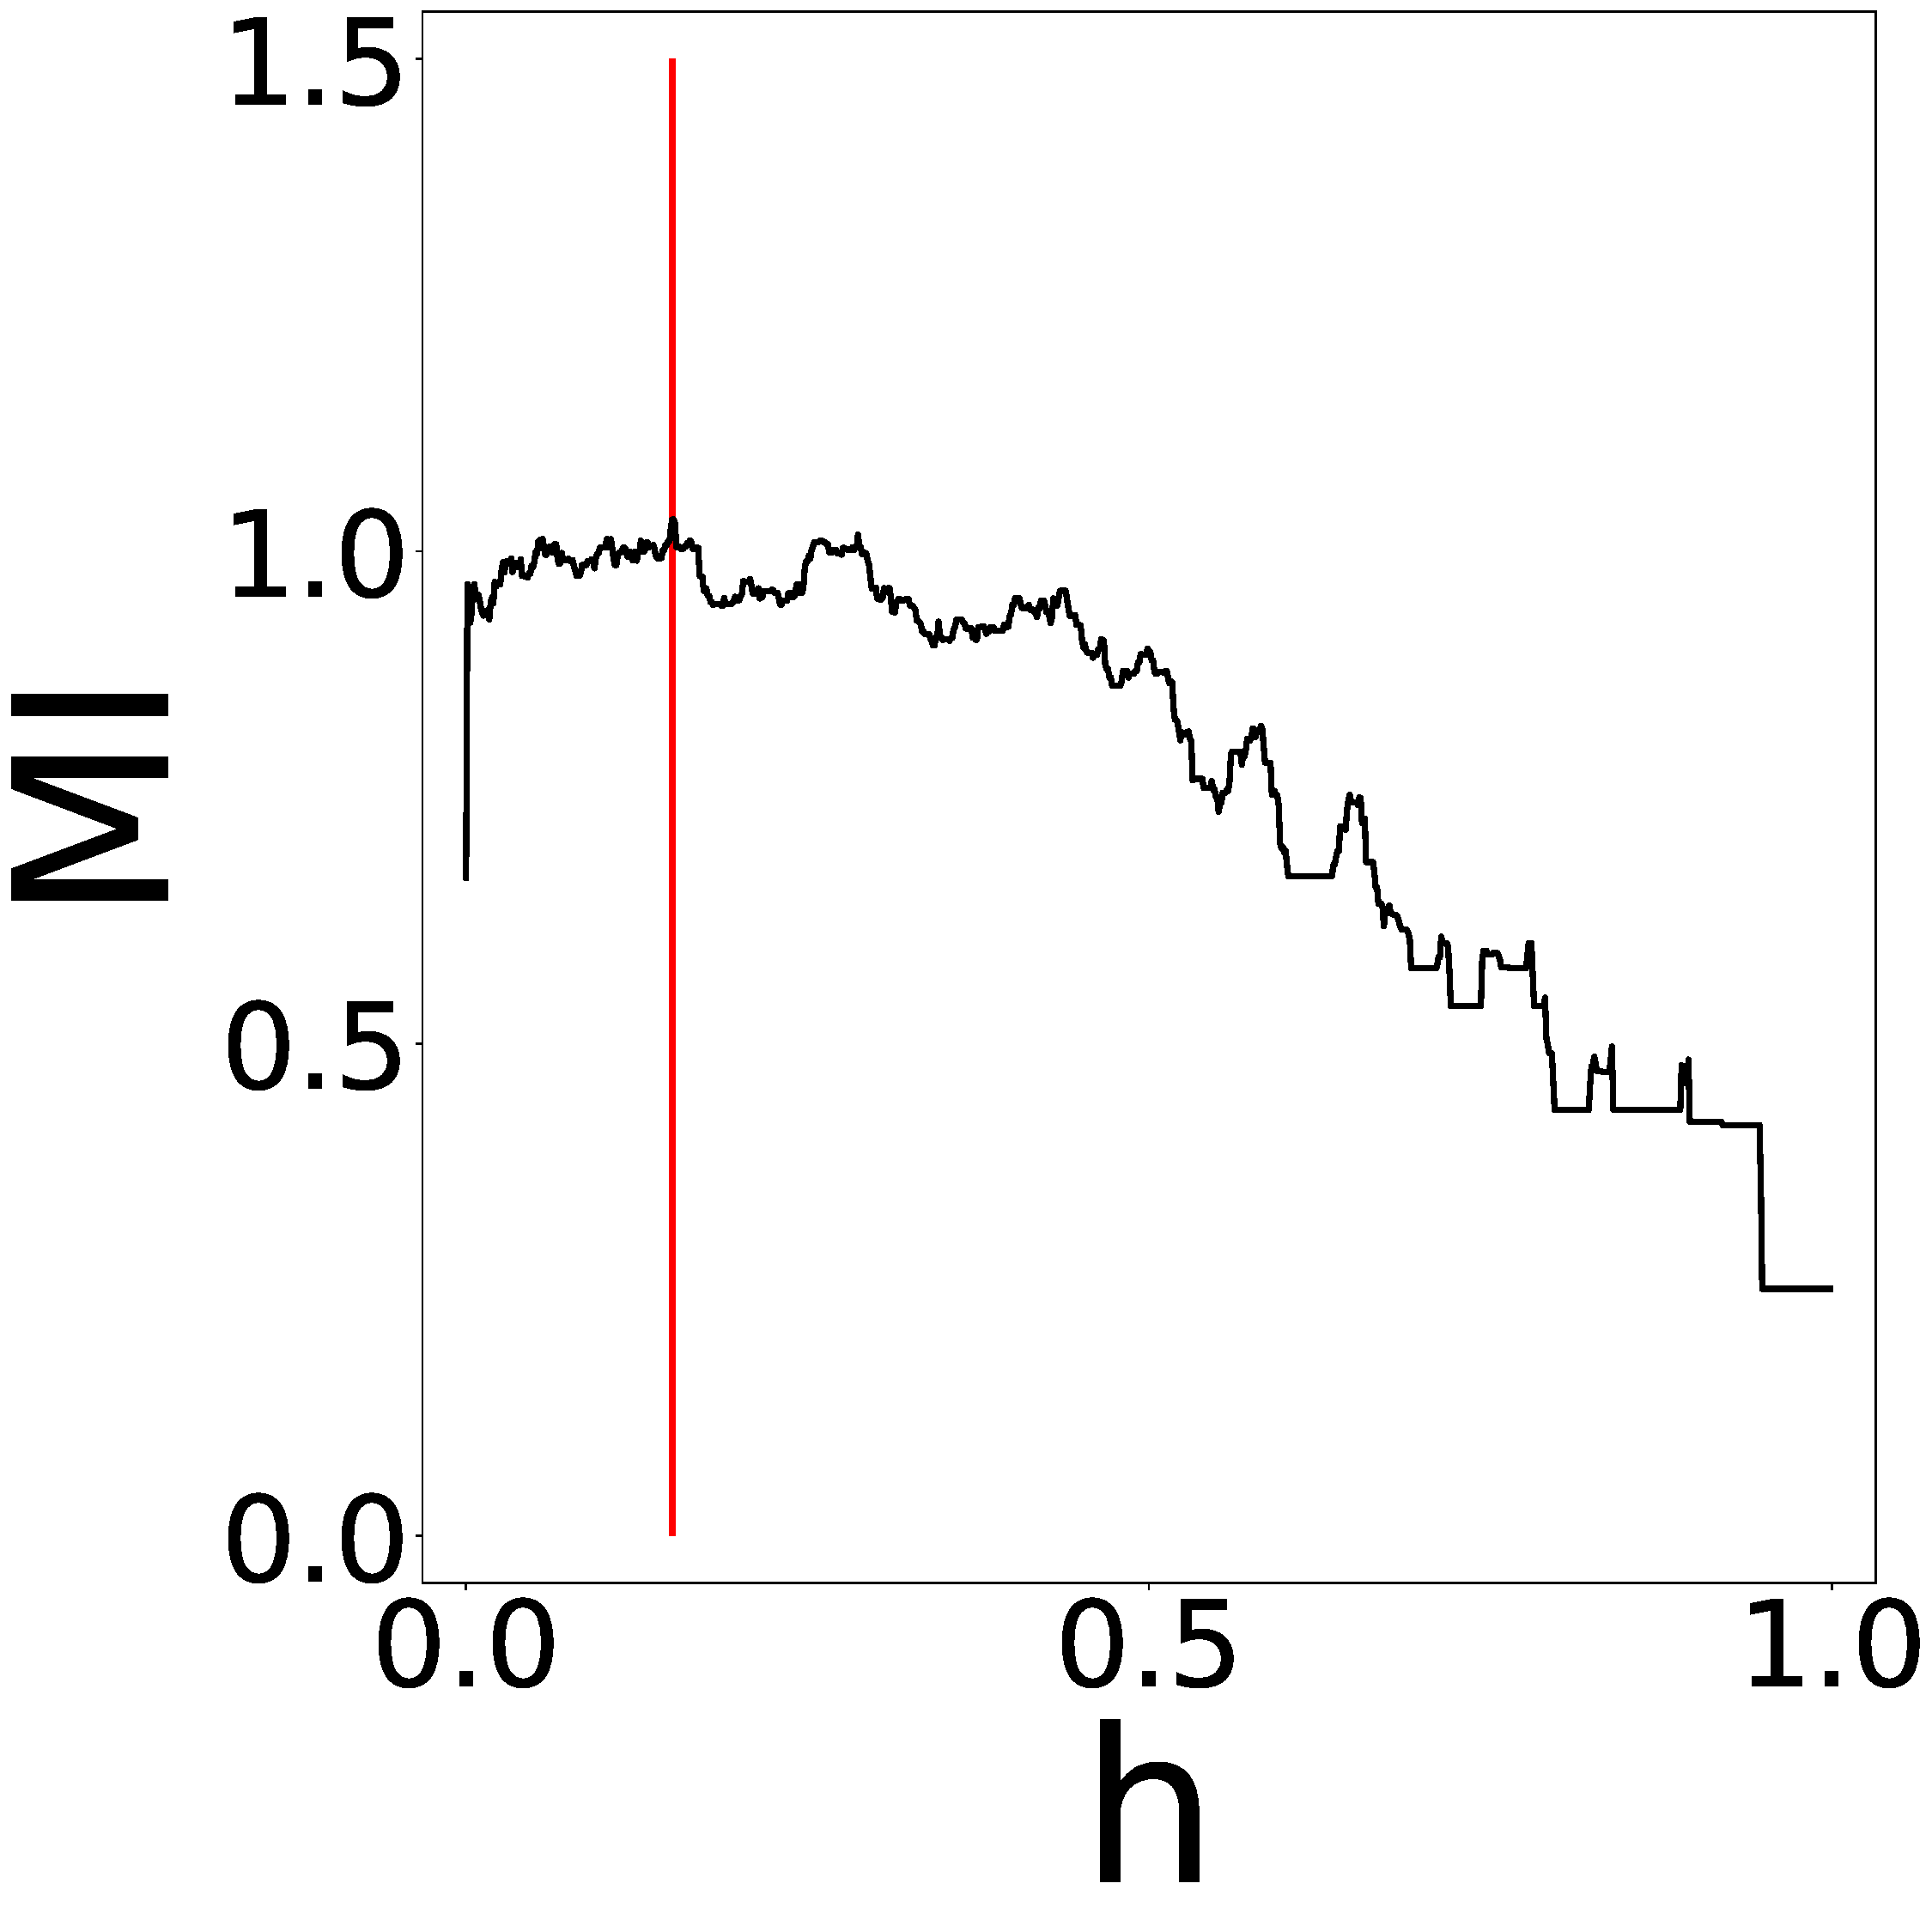
\includegraphics[width=0.25\linewidth]{5_A_h_va}};
\node [anchor=north west]  (img4) at (0.26\linewidth,.618\linewidth){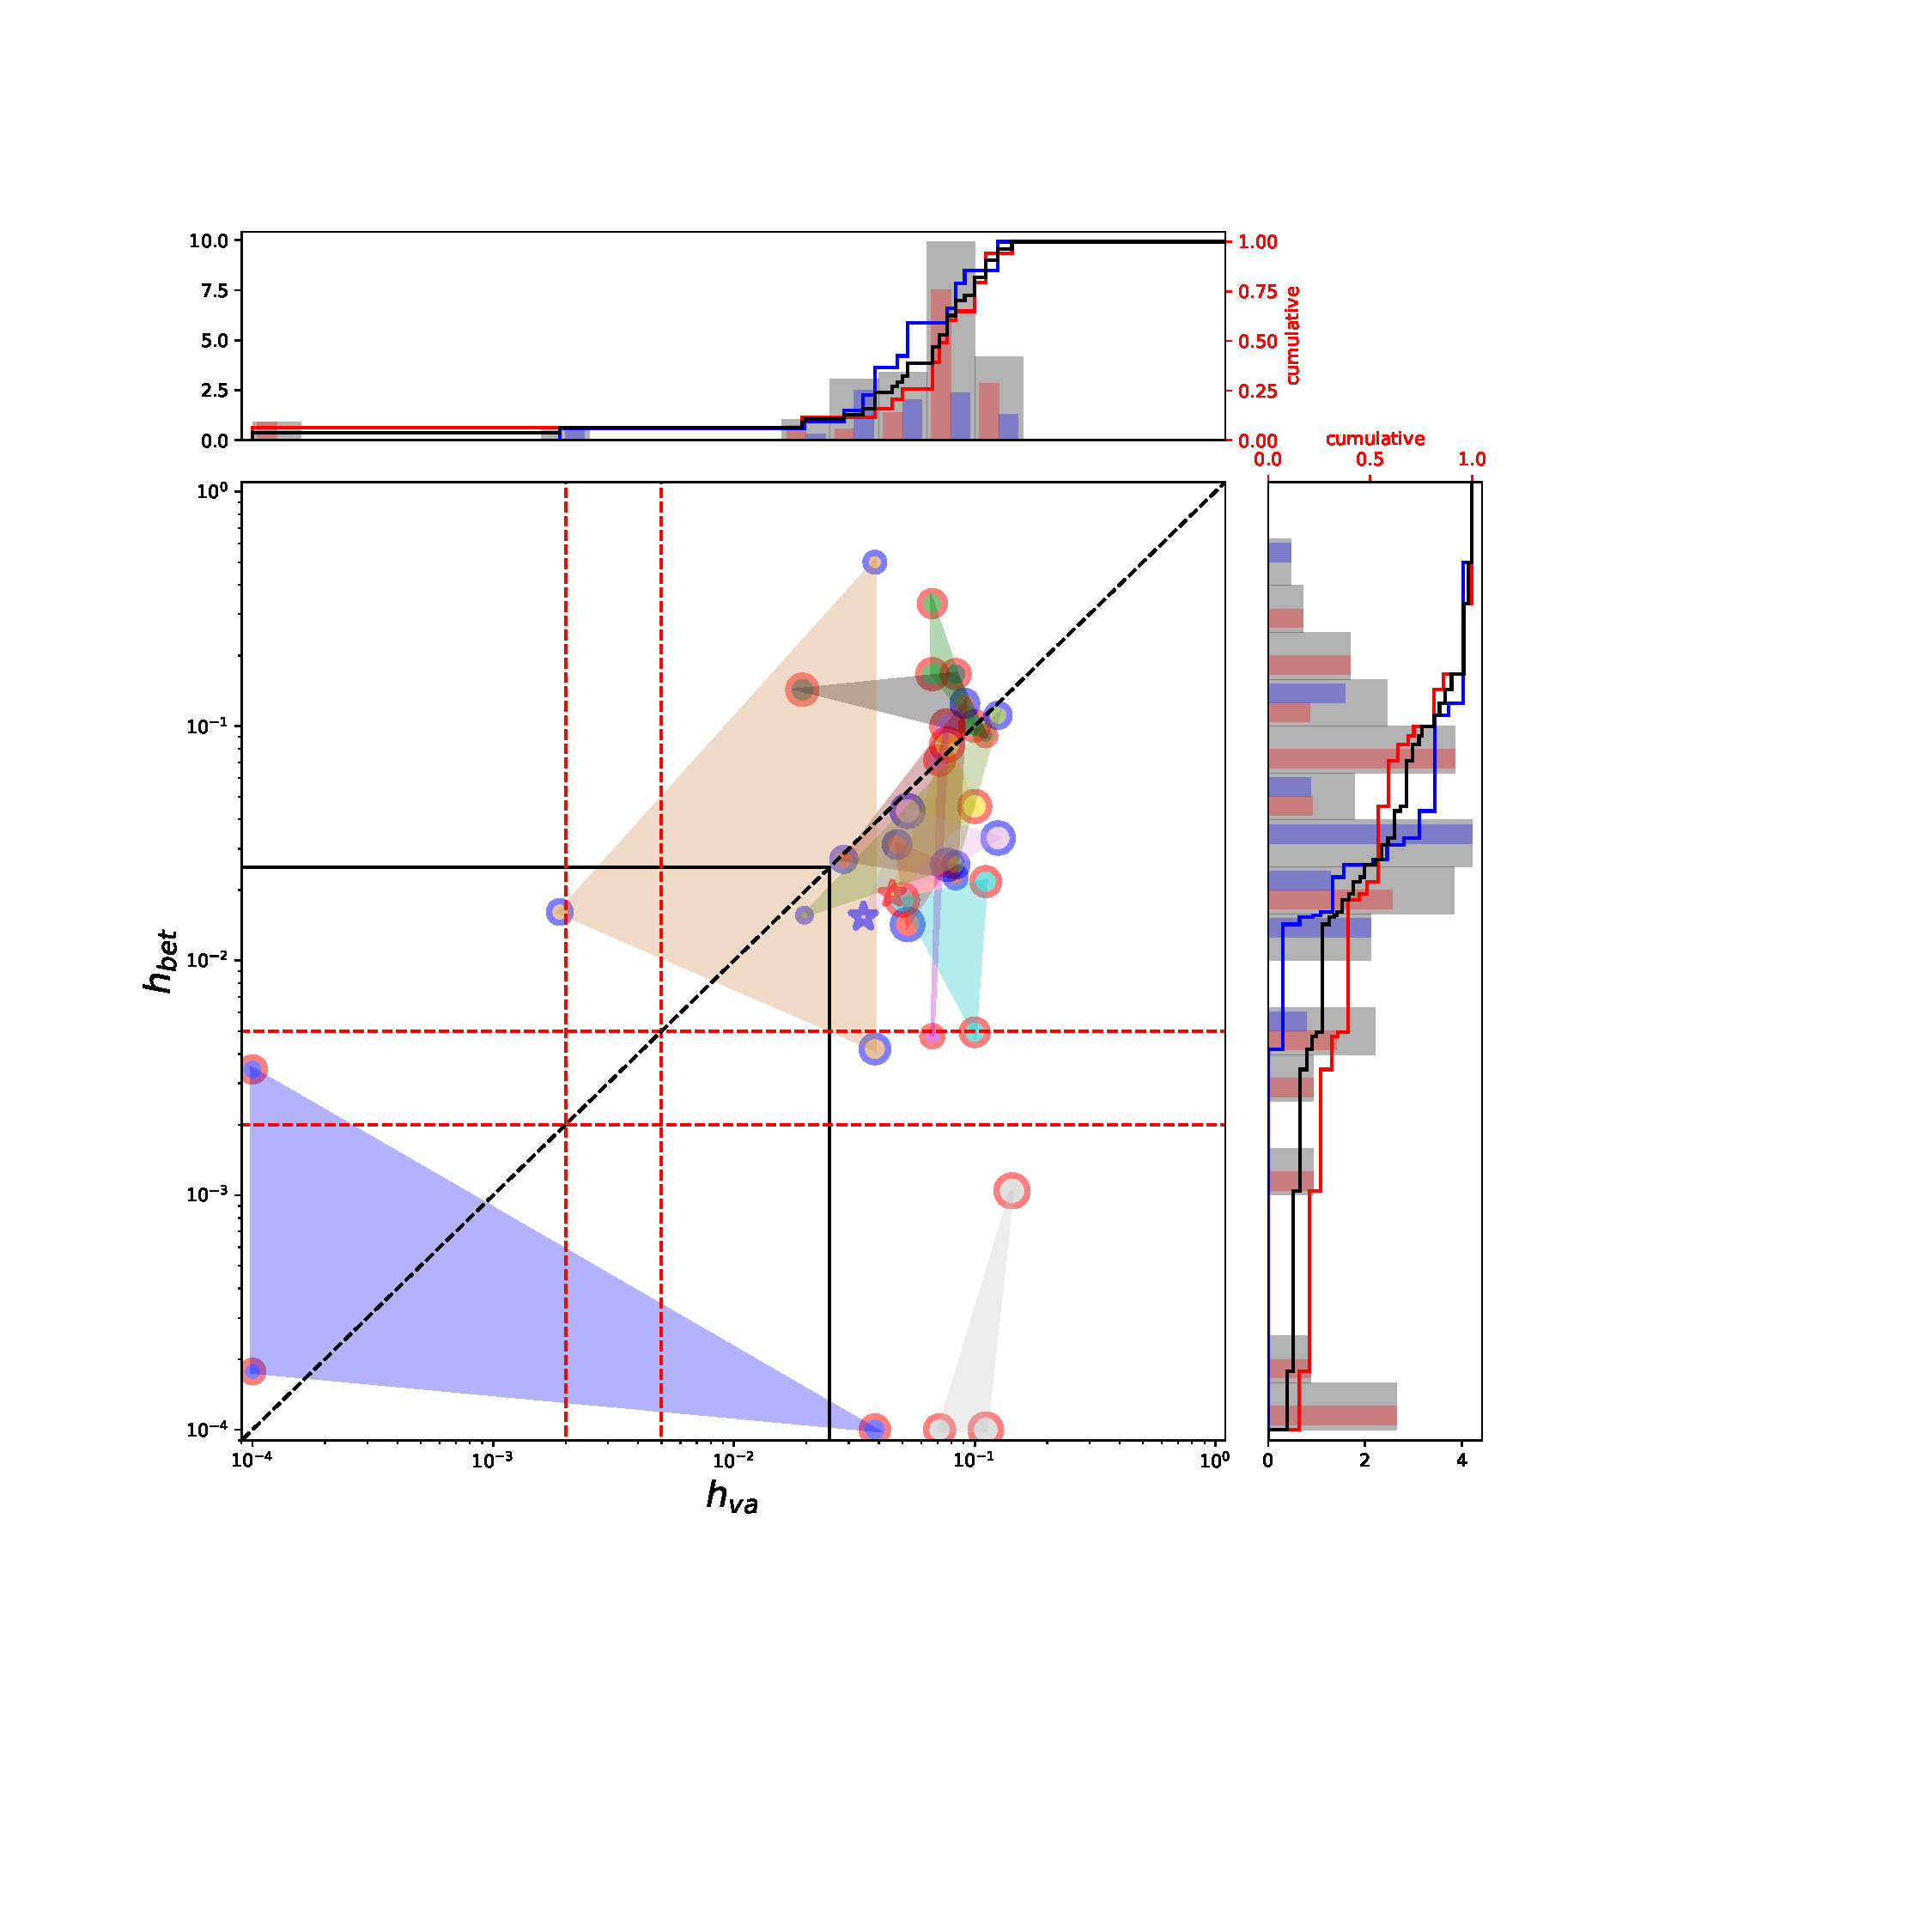
\includegraphics[width=0.618\linewidth]{5_inter-individual_differences_fit}};
%
%\draw [anchor=north west] (0.000\linewidth, .618\linewidth) node {$\mathsf{(A)}$};
%\draw [anchor=north west] (0.25\linewidth, .618\linewidth) node {$\mathsf{(B)}$};
%
\end{tikzpicture}
}


%\begin{figure}%[b!]
%\begin{center}
%  %\includegraphics[width=1\linewidth]{figure5}
%
%  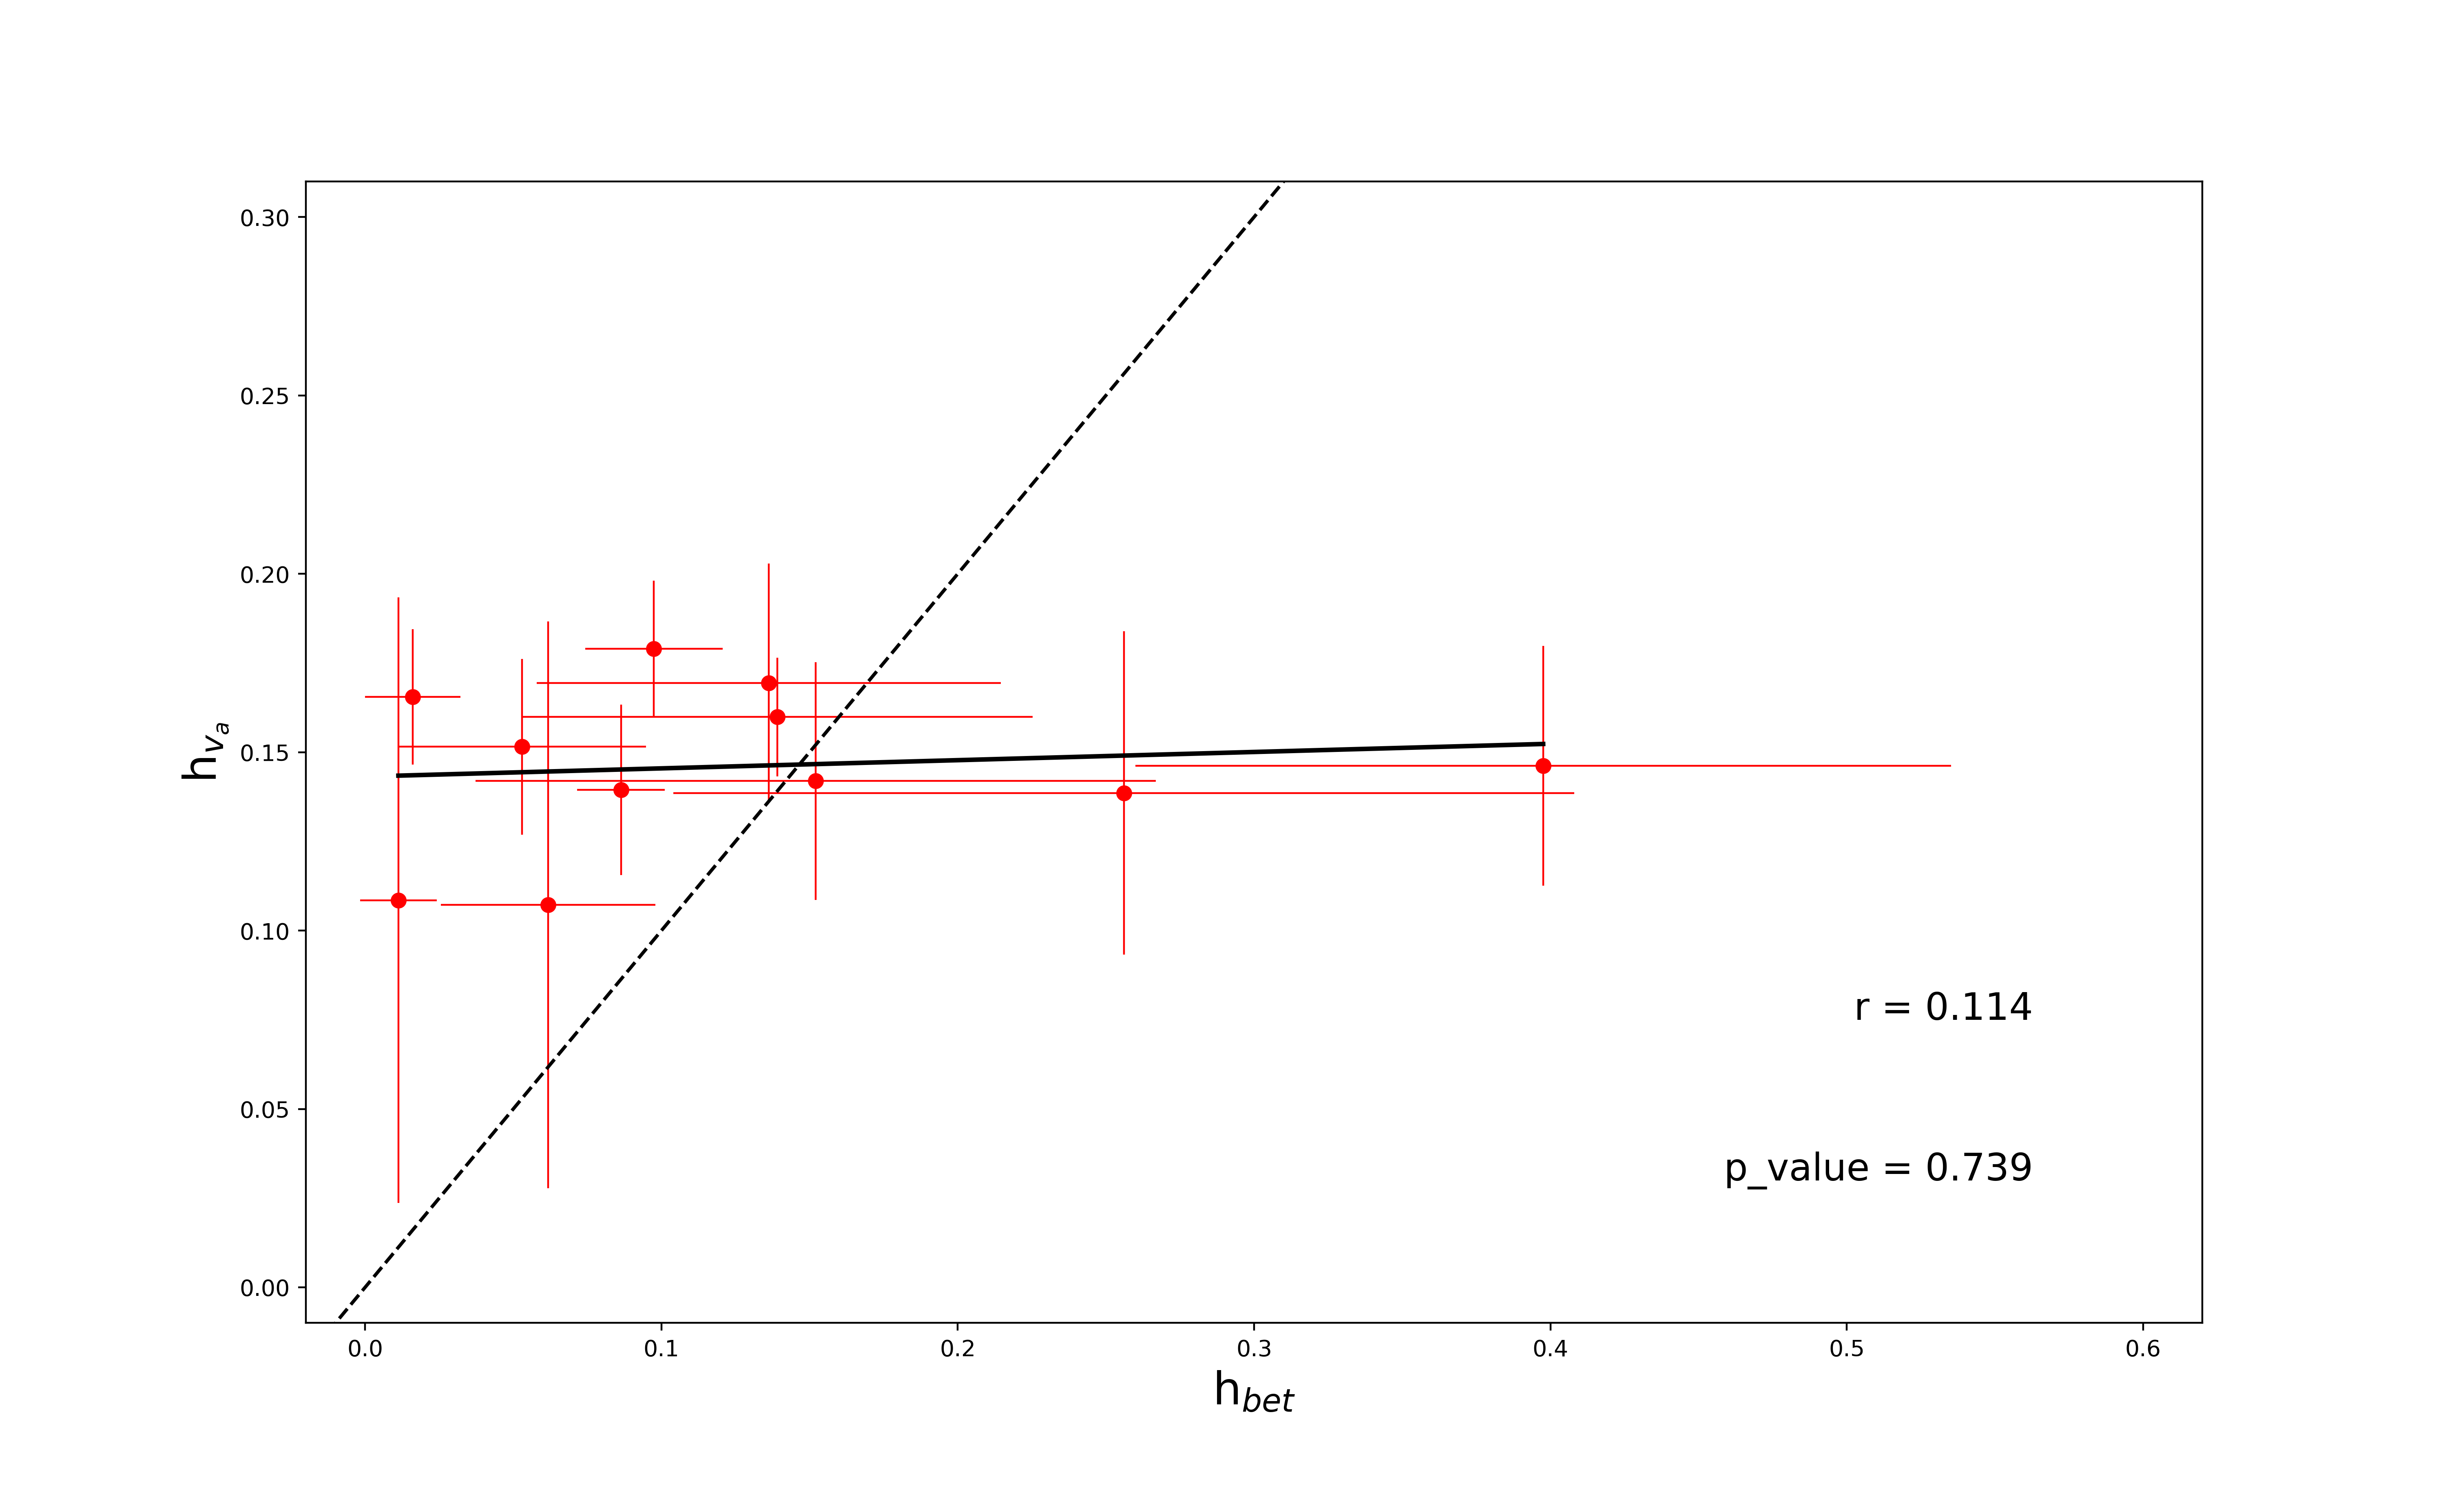
\includegraphics[width = 1 \linewidth]{5_inter-individual_differences}
%\end{center}
\caption{\emph{Analyzing inter-individual differences}
\textbf{(A)}
\LP{ show fit with different hazard rates for one observer / one block}
\CP{sujet IP 2eme block,  en haut: MI entre les bet et le bcp pour les differents h, en bas: MI entre les vitesse d'anticipation et le bcp pour different h}
% TODO compare with the results you would obtain from a fixed window fit.
\textbf{(B)}
result of fits for different observers / SEM across blocks
\CP{il y a aussi la figure pour les h selectiones avec le MI (5 inter individual differences MI)}
}
\label{fig:results_inter}
\end{figure}
%-------------------------------------------------------------%
Hence, we have fitted the sequence of responses generated by each participant and
for each session, that is for the eye movements and the rating scale experiments.
The scatter plot of the best fit values are shown in~\seeFig{results_inter}.
This figure suggests, in the first place, that there is some variability in the best fit value of $\tau$
in both sessions.
If the average is close to the (hidden) value used to generate the sequence
(with $\tau = XX~\ms \pm XX~\ms$ for the first session and
 $\tau = XX~\ms \pm XX~\ms$ for the second),
 we observe a variability which is characteristic of the spectrum of individual choices.
More importantly, there is a small but consistent
correlation between the individual best-fit values estimated for the first and the second session.
% TODO - Granger / transfer entropy
Also we have found that using measures of causality %\AM{COOL!}, LP: yaka :-)
the results for eye movements slightly lagged before
that of the rating scale,
suggesting that there could be an advance
It can serve as a biomarker...

%: %%%%%%%%%%%%%%%%%%%%%%%%%%%%%%%%%%%%%%%%%%%%%%%%%%%%%%%%%%%%%%%

\section{Discussion}

\label{sec:outro}

%The oculomotor system has to constantly update its knowledge about the environment. An ordeal is then to adapt to changes with the shortest delays. Early studies have proposed that stimuli provides information to modulate reaction times within sequences~\citep{Hyman1953, Tune1964, Schvaneveldt}. This theoretical approach is coherent with the notion of local transition probabilities that quantifies at which extent an observation deviates from the preceding ones~\citep{Meyniel16}. The way expectations act on cognitive processes has been investigated by a wide range of domains such as predictive coding~\citep{Wolpert2000, Wacongne2012}, active inference~\citep{Friston2010}, motor control~\citep{Sutton1998, Behrens07} and reinforcement learning~\citep{Nassar2012}. Non-stationary observations can also explain why both local and global effects emerge and why local effects persist in the long run even within purely random sequences~\citep{Cho2002, Yu2009}. This constant update of a general belief on the world can be a consequence of the constant attempt to learn the non-stationary structure of the environment that can change at unpredictable times~\citep{Yu2009}. Many studies have actually already pointed the brain's ability to apprehend non-stationary states in environments~\citep{Ossmy2013, Meyniel15}. As explained by~\citet{Meyniel16}, the belief upon an environment can be divided in two different ways:
%
%\begin{enumerate}[label=\Alph*)]
%\item Update the~\textit{a priori} likelihood of a sudden change, also known as the volatility and taken into account by the model~\citep{Behrens07}
%\item A leaky integrator factor imbedded in the model~\citep{Anderson2006, Yu2009, Ossmy2013, Wang2002}
%\end{enumerate}
%

%: theory / computationnally-driven experiments
% it's a main novelty
generative models for changing environments allows to know the ground truth compared to natural stimulation (see Rust eand Movshon)%
Let's remember our hierarchical generative model.

At any given trial, we wish to construct an algorithm which

We will introduce a fundamental component of Bayesian models : a latent variable

this new variable will be used to test different hypothesis which will be evaluated to predict future states. it is called latent because it aims at representing a variable that is latent (or hidden) to the observer

in our case, we will assume that the Bayesian model knows about the structure of the generative model and we will set it to the current run-length $r$, that is, at any given trial, the hypothesis that the past r observations belong to the same block. of course a wrong choice of a latent variables (let's say the temperture in the experimental room) may give unexpected results, even is the Bayesian model is ``optimal'' - an essential point to understand in Bayesian inference

extension to multi-nomioal( daniele + fred danion)



% Still, only Bayesian models recover an explicit probabilistic representation of change in likelihood. Recent experimental studies suggest, indeed, that the brain is able of estimating a hierarchical model of the environment and that humans can explicitly report sudden changes in sequences~\citep{Meyniel15, Gallistel2014}. Ultimately, we passed over one of leaky integrator models' main default, having a too fixed and rigid memory parameter. In our work the memory parameter is constantly inferred by the BBCP algorithm over the observation of the number of trials where this inference stayed reliable and then globally represented probabilistic representation of changes in likelihood and actualization of~\textit{a priori} knowledge.


perspectives:
- RL : use hindsight example of localization for saccades: get the changepoints then improve estimate of reward allows to optimize the association between the set of measures and their utility (compared to Q-learning where it is a fixed length)
- interindividual differences : markers for the berhaviour traces - traces of the network implementation / testing different h
- the brain is weakly Bayesian (it does not care about equations but more about sugar)


One remaining question though, is to understand why in cognitive systems
this adaptation occurs and
in particular why it may deviate
in some pathological disorders such as schizophrenia~\citep{Adams12}.

%: %%%%%%%%%%%%%%%%%%%%%%%%%%%%%%%%%%%%%%%%%%%%%%%%%%%%%%%%%%%%%%%

\section{Conclusions}


\begin{itemize}\setlength{\itemsep}{0ex}
\item \AM{ We observed a good correlation between the largely unconscious anticipatory smooth eye movements and the explicit rating of confidence on expected stimulus motion direction },
\item There is a strong correlation between the real probability and the value of the direction confidence rating,

\item there is a stong correlation between the strength of anticipation and the probability of the process,

\item we have developed a Bayesian model of an agent estimating the probability of changing points. This allows to dynamically infer the direction probability and directly compare model and human behaviour.
\item \AM{ The quality of the correlation with the experimental measures (confidence rating and anticipatory eye movements) is enhanced when the model-predicted direction bias $\hat{p}$ is taken as regressor instead of the real probability bias, suggesting that this model captures some of the brain computations underlying expectancy based motion prediction},
\item \AM{CONCLUSION on individual differences?}


% to summarize, we have shown that
% - there is a correlation in the anticiapatory response of eye movements
% in a volatile environment that is captured if we know the true probability
% - that a fixed length models captures some of this correlation, but that
% - our online bayesian changepoint model better captures this correlation
% and that this may hint at the neural mechanisms used to anticipate
% in a dynamic environment
%
% the brain is not strongly a bayesian machine, but weakly

\end{itemize}
%: %%%%%%%%%%%%%%%%%%%%%%%%%%%%%%%%%%%%%%%%%%%%%%%%%%%%%%%%%%%%%%%
\section{Material and Methods}
%%%%%%%%%%%%%%%%%%%%%%%%%%%%%%%%
%%%%%%%%%%%%%%%%%%%%%%%%%%%%%%%%
\subsection{Participants, visual stimuli and experimental design}
%%%%%%%%%%%%%%%%%%%%%%%%%%%%%%%%
Twelve observers (29 years old +/- 5.15 \AM{, XX females}) with normal or corrected-to-normal vision took part in these experiments. They gave their informed consent and the experiments had received ethical approval from the Aix-Marseille Ethics Committee (approval 2014-12-3-05), in accordance with the declaration of Helsinki.

Visual stimuli were generated using PsychoPy 1.85.2 on a Mac running OS 10.6.8 and displayed on a 22" Samsung SyncMaster 2233 monitor with $1680\times 1050$ pixels resolution at 100~\si{\Hz} refresh rate. Experimental routines written using PsychoPy 1.85.2 controlled the stimulus display. Observers sat 57~\si{\cm} from the screen in a dark room. 

The moving target used in our experiments was CHECK: a white ring ($0.35\degree$ outer diameter and $0.27\degree$ inner diameter) with a luminance of 102 cd/m2 that moved horizontally on a grey background (luminance $42cd/m^2$). Each trial started with a central fixation point displayed for a random duration drawn from a uniform distribution ranging between 400 and 800ms. Then a fixed-duration 300ms gap occurred between the offset of the fixation point and the onset of the moving target, which was presented slightly offset from the fixation location (\citet{Rashbass1961}) and immediately started moving horizontally at a constant speed of $15\degree/s$, either to the right or to the left for 1000 ms. The probability P of rightward trials was a time-varying random variable which was constant within a sub-block of the sequence of a given random size (See Figure  and main text for the description of the generative model). 

The paradigm included two experiments performed on two consecutive days by each participants and involving the presentation of the same sequence of trials, while collecting a different behavioral response, the \textit{Eye movements} and the \textit{Explicit prediction} (or \textit{Bet}) experiments. Asked after the experiment, no observer noticed that the same (pseudo-)random sequence of target directions was used in both experiments.

\subsection{Eye movements experiment}
Eye movements were recorded continuously with an eye tracking system (Eyelink 1000, SR Research Ltd., sampled at 1000 Hz), using the Python module Pylink 0.1.0. Horizontal and vertical eye position data were transferred, stored, and analyzed offline using programs written in Ipython notebooks.
To minimize measurement errors, the subject's head movements were restrained using a chin and forehead rest, so that the eyes in primary gaze position were directed towards the center of the screen. In order to enforce accuracy in gaze position and tracking, we implemented an automatic procedure of fixation control. If the distance between the gaze position and the central fixation point during the fixation epoch exceeded $2\degree$ of visual angles, the fixation point started flickering and the counter for the fixation duration was reset to $0$. 

The recorded horizontal and vertical row gaze position data were numerically differentiated to obtain velocity measures \AM{any other details?}. We adopted an automatic conjoint acceleration and velocity threshold method (the default saccade detection implemented by SR Research) to detect ocular saccades. Saccades and eye-blinks were excluded from eye velocity traces (and replaced by NaN values in the numerical arrays) before trial averaging. 
In order to extract the relevant parameters of the oculomotor responses, we developed new tools based on a best-fitting procedure of predefined oculomotor patterns and in particular the typical smooth pursuit velocity profile that was recorded in our experiment (Top row). This analysis was applied to each trial individually and it allowed in particular to estimate the anticipatory smooth pursuit velocity. More details abut the oculomotor data processing and parameter extraction are provided in Appendix \ref{app:em} 

The python scripts used to analyse eye movements are available at \url{https://github.com/invibe/ANEMO}.

\subsection{The Bet experiment}
The aim of the second experiment (occurring the following day after the Eye Movement experiment) was to collect data related to the individual conscious estimate of the probability of target motion direction. At the beginning of each trial, before the presentation of the moving target, participants had simply to answer to the question \textit{ ``How sure are you that the target will go left or right''}. This was performed by adjusting a cursor on the screen using the mouse (see Figure~\seeFig{intro}-C). The cursor could be placed at any point along a horizontal segment representing a linear rating scale with three ticks labeled as \textit{ ``Left''}, \textit{``Right''} (at the extreme left and right end of the segment respectively), and \textit{``Unsure''} in the middle. Participants had to validate their choice by clicking on the mouse left-button and the actual target motion was shown thereafter. The rationale to collect rating responses on a continuous scale instead of a simple binary prediction (Right/Left) was to be able to infer the individual estimate of the direction bias at the single trial scale (in analogy to the continuous interval for the strength of aSPEM velocity).

We called this experiment the \textit{ ``Bet''} experiment, as subjects were explicitly encouraged to make reasonable rating estimates, as though they had to bet money on the next trial outcome. Every $50$ trials, a \textit{``score''} was displayed on the screen, corresponding to the proportion of correct direction predictions (Right or Left of the \textit{``Unsure''} tick) weighted by the confidence attributed to each answer (the distance of the cursor from the center).


%\subsection{Eye movements analysis}
%The data analyses were implemented using the Python libraries numpy, pandas and pylab. All the scripts for data analysis, as well as for stimulus presentation, data collection, and preparation of figures are available on github at \url{https://github.com/chloepasturel/AnticipatorySPEM}.
 

%%%%%%%%%%%%%%%%%%%%%%%%%%%%%%%%
%: %%%%%%%%%%%%%%%%%%%%%%%%%%%%%%%%%%%%%%%%%%%%%%%%%%%%%%%%%%%%%%%
\section{Appendices}
%%%%%%%%%%%%%%%%%%%%%%%%%%%%%%%%
%%%%%%%%%%%%%%%%%%%%%%%%%%%%%%%%
\subsection{Appendix 1: Analysis of eye movements}
\label{app:em}
%%%%%%%%%%%%%%%%%%%%%%%%%%%%%%%%


%: FIGURE 1B fig:introB ~\seeFig{introB}
\begin{figure}%[b!]
\centering{
%\includegraphics[width=\linewidth]{figure1}
\begin{tikzpicture}%[thick,scale=1, every node/.style={scale=1} ]
\node [anchor=north west]  (img2) at (0.51\linewidth,.33\linewidth){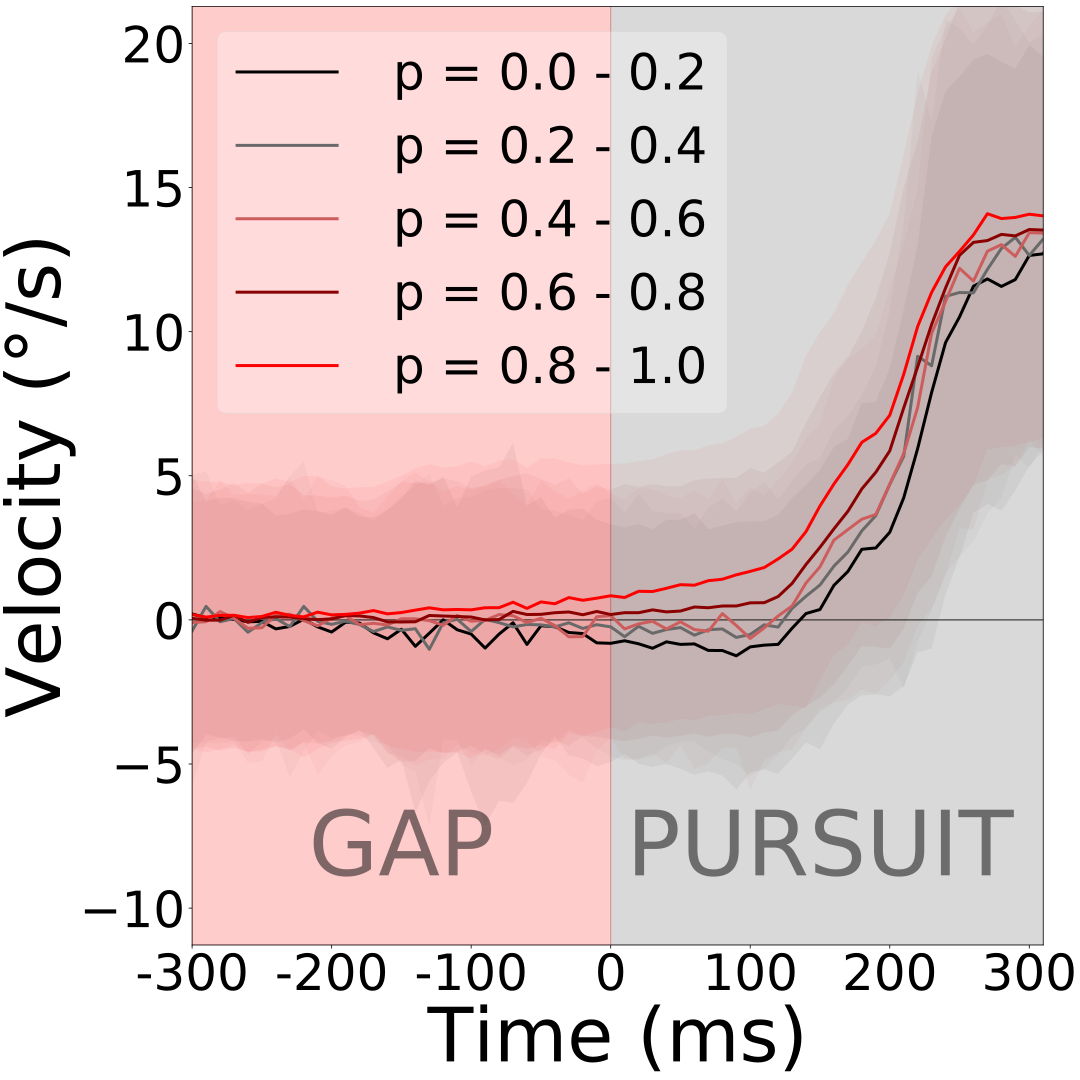
\includegraphics[width=0.33\linewidth]{1_B_Trace_moyenne}};
%\draw [anchor=north west] (0.000\linewidth, .62\linewidth) node {$\mathsf{(A)}$};
%\draw [anchor=north west] (0.505\linewidth, .62\linewidth) node {$\mathsf{(B)}$};
\end{tikzpicture}
}
\caption{
%\emph{Anticipatory SPEM (aSPEM): experimental design and results.} 
%\textbf{(A)}~TODO: MOVE THIS PART IN THE MAIN TEXT:
\emph{Behavioral experiments: anticipatory Smooth Pursuit Eye Movements}
% TODO : dans notre plot on a des range de valeurs pour p :-/ -> C'EST PARCE QUE LE PLOT REPRESENTE DEJA LA VITESSE MOYENNE OBTENUE DANS LA TACHE AVEC SWITCHES!
%\textbf{(B)}~
We first replicated the results of~\citet{Montagnini2010},
in which human observers were presented with several $500$ trials blocks of horizontal target motion with a block-dependent direction probability bias, and they were asked to track the target with their gaze.
An important difference with that study is that their experiment was made of several blocks of target motion with a block-dependent direction probability bias selected among a few predetermined values, whereas in the present study $p$ can change in each different block as a random number between $0$ and $1$.
Horizontal eye velocity traces 
averaged, over rightward trials and all observers, for five different intervals of the direction bias.
These traces are aligned to the onset of the moving dot (the $0$ on the $x-axis$).
Saccades were removed using a thresholding method~(see~\seeApp{em}) and
the shaded area around the traces represent one standard deviation over all velocity samples.
In the unbiased or weakly biased condition ($0.4\leq p\leq 0.6 $), one can distinguish
a visually-driven component (after a latency of $\approx 100~\ms$)
which corresponds to the standard Smooth Pursuit Eye Movement (SPEM) initiation.
When introducing a bias in the direction,
the average eye velocity progressively ramps
in the direction of the expected velocity, starting during the GAP phase and well before the visually-driven component:
This phase is the anticipatory SPEM (aSPEM).
As previously reported~\citep{Montagnini2010, SantosKowler2017,Damasse18},
the slope of this ramp correlates with the strength of the bias.
In this study, we extended this experiment in three aspects.
First, we used probability biases in a continuous space,
as drawn from a prior distribution for the values of $p$.
Second, we generated the random sequence of trials
by concatenating random-length blocks (see \seeFig{results_psycho}),
to avoid potential confounds related to the previously used blocked-design.
}
\label{fig:introB}
\end{figure}


I show here a typical velocity traces for one subject / 2 trials

- x-axis is time in milliseconds aligned on target onset,
and we show respectively from left to right the fixation in gray,
the GAP in pink (300ms) and the run in light gray.

- y-axis is the velocity as computed as the gradient of position.
Remark that the eyelink provides with the periods of saccades or
 blinks that we removed from the signal. it is quite noisy and
 to complement existing signal processing methods,
 Chloe implemented a robust

- fitting method which allows to extract some key components of
the velocity traces: maximum speed, latency, temporal inertia ($\tau$)
 and most interestingly acceleration before motion onset.
 We cross-validated that this method was giving similar results
  to other classical methods but in a more robust fashion/

While being sensible to recording errors, this allows us to extract the
 anticipatory component of SPEMs and..

%%%%%%%%%%%%%%%%%%%%%%%%%%%%%%%%
\subsection{Appendix : leaky integrator}
\label{app:leaky}
Given a series of observations $\{x_0^i\}_{0\leq i \leq t}$
with $\forall i, x_0^i \in \{0, 1 \}$, we defined
\eqs{
\hat{x_1}^{t} &= 1/\tau \cdot \sum_{0\leq i \leq t} (1 - 1/\tau)^{i} \cdot x_0^{t-i}\\
			  &= h \cdot \sum_{0\leq i \leq t} (1 - h)^{i} \cdot x_0^{t-i}
}
%is true for $t=1$: by definition $\hat{x_1}^{0}=x_0^0$ and
%\eq{
%\hat{x_1}^{1} = (1 - \rho) \cdot \hat{x_1}^{0} + \rho \cdot x_0^1
%}
If we write it for trial $t-1$, we have
\eqs{
\hat{x_1}^{t-1}	&= h \cdot \sum_{0\leq i \leq t-1} (1 - h)^{i} \cdot x_0^{t-1-i} \\
                &= h \cdot \sum_{1\leq j \leq t} (1 - h)^{j-1} \cdot x_0^{t-j} \\ % j = i+1
(1 - h) \cdot \hat{x_1}^{t-1} &= h \cdot \sum_{1\leq i \leq t} (1 - h)^{i} \cdot x_0^{t-i}
                }
As such, the relation
\eqs{
\hat{x_1}^{t}	&= h \cdot \sum_{0\leq i \leq t} (1 - 1/\tau)^{i} \cdot x_0^{t-i} \\
				&= h \cdot x_0^{t} + h \cdot \sum_{1\leq i \leq t} (1 - h)^{i} \cdot x_0^{t-i} \\
				&= h \cdot x_0^{t} + (1 - h) \cdot \hat{x_1}^{t-1} \\
}
such that finally
\eq{
\hat{x_1}^{t} = (1 - h) \cdot \hat{x_1}^{t-1} + h \cdot x_0^t
}
As such, the definitions in~\seeEq{leaky} and ~\seeEq{leaky2} are equivalent.
%%%%%%%%%%%%%%%%%%%%%%%%%%%%%%%%
\subsection{Appendix 2: BBCP algorithm}
\label{app:bcp}

%to represent our belief at trial $t$
%or to determine the pdf for $x_1^t$ as a mixture of Beta distributions:
%\eqa{
%\hat{x_1}^{t} =  \sum_{r^{t}} Pr(x_1^t | r^{t}, x_0^{0:t}) \cdot Pr(r^{t} | x_0^{0:t})
%}


To summarize, the algorithm that we presented
% TODO: show as python code
%* an implementation of
%%[Adams &amp; MacKay 2007 "Bayesian Online Changepoint Detection"](http://arxiv.org/abs/0710.3742)
%in Python.
%
%
%* adapted from https://github.com/JackKelly/bayesianchangepoint by Jack Kelly (2013) for a binomial input.
%
%* This code is based on the  [MATLAB implementation](http://www.inference.phy.cam.ac.uk/rpa23/changepoint.php) provided by Ryan Adam. Was available at http://hips.seas.harvard.edu/content/bayesian-online-changepoint-detection
%
% * full code @ https://github.com/laurentperrinet/bayesianchangepoint are available at \url{https://github.com/laurentperrinet/bayesianchangepoint}.

Knowing $p$ and $r$, the sufficient statistics of the beta distribution $B(\alpha, \beta)$ :


\subsubsection{The binomial and Beta distributions}

binomial
\eq{
\Pr(k;n,p) = \Pr(X = k) = {n\choose k}p^k(1-p)^{n-k}
}


Bernoulli $p(x | p) = p^x \cdot (1-p)^{1-x}$
%TODO say Bernoulli instead of binomial when just one draw
Wikipedia: For example, the beta distribution can be used in Bayesian analysis to describe initial knowledge concerning probability of success such as the probability that a space vehicle will successfully complete a specified mission. The beta distribution is a suitable model for the random behavior of percentages and proportions.

conjugate is the Beta-distribution of shape parameters $\alpha = p\cdot r$ and $\beta = (1- p)\cdot r$:
$ P(p | \alpha, \beta ) = \frac{1}{B(\alpha, \beta)} \cdot p^{\alpha -1} \cdot (1-p)^{\beta - 1} $

\eqs{
        \alpha &= p*r \\
        \beta  &= (1-p)*r
    }
inversely, $\alpha + \beta = r$ and $p = \frac{\alpha}{\alpha +\beta} = 1- \frac{\beta}{\alpha + \beta}$
%var = \frac {\alpha-1}{(\alpha +\beta+2)\cdot(\alpha +\beta+3)}$



\subsubsection{Initialization}

	\begin{itemize}
		\item    $P(r_0)= S(r)$ or $P(r_0=0)=1$ and
		\item    $\mu^{(0)}1 = \mu_{prior}$ and $\nu^{(0)}1 = \nu_{prior}$
	\end{itemize}

Note that the prior distribution is a Beta distribution:
$\Pp\propto B(p; \mu_{prior}, \nu_{prior})$.
It will by symmetry be unbiased: $\mu_{prior}=.5$.
Concerning the shape, it can be for instance
the uniform distribution $\Uu$ on $ [ 0, 1 ] $, that is $\nu_{prior}=2$ or
Jeffrey's prior $\Jj$, that is $\nu_{prior}=1$.

%Wikipedia: Beta(1/2, 1/2): The arcsine distribution probability density was proposed by Harold Jeffreys to represent uncertainty for a Bernoulli or a binomial distribution in Bayesian inference, and is now commonly referred to as Jeffreys prior: p−1/2(1 − p)−1/2. This distribution also appears in several random walk fundamental theorems

\subsubsection{Update}

    Observe New Datum $x_t$,

\subsubsection{Prediction: run-length distribution}

\eqs{
%\hat{x_1}^{t} =
Pr(x_0^t | x_0^{0:t-1}) &= \sum_{r^{t}} Pr(x_0^t | r^{t}, x_0^{0:t-1}) \cdot  \beta^{(r)}_t \\
Pr(x_0^t | x_0^{0:t-1}) &= \sum_{r^{t}} Pr(x_0^t | r^{t}, x_0^{0:t-1}) \cdot  Pr(r^{t} | x_0^{0:t-1})\\
\text{with} \quad Pr(r^{t} | x_0^{0:t-1}) &\propto \sum_{r^{t-1}}  Pr(r^t | r^{t-1}) \cdot  Pr(x_0^t | r^{t-1}, x_0^{0:t-1}) \cdot  Pr(r^{t-1} | x_0^{0:t-2})
\text{with} \quad \beta^{(r)}_t &\propto \sum_{r^{t-1}}  Pr(r^t | r^{t-1}) \cdot  Pr(x_0^t | r^{t-1}, x_0^{0:t-1}) \cdot  \beta^{(r)}_{t-1}
}


\begin{enumerate}

\item    Evaluate Predictive Probability $\pi_{0:t} = P(x_t |\mu^{(r)}_t,\nu^{(r)}_t)$.
    \item    Calculate Growth Probabilities $P(r_t=r_{t-1}+1, x_{0:t}) = P(r_{t-1}, x_{0:t-1}) \pi^{(r)}_t (1-H(r^{(r)}_{t-1}))$,
    \item    Calculate Changepoint Probabilities $P(r_t=0, x_{0:t})= \sum_{r_{t-1}} P(r_{t-1}, x_{0:t-1}) \pi^{(r)}_t \cdot H(r^{(r)}_{t-1})$,
    \item    Calculate Evidence $P(x_{0:t}) = \sum_{r_{t-1}} P (r_t, x_{0:t})$,
    \item    Determine Run Length Distribution $P (r_t | x_{0:t}) = P (r_t, x_{0:t})/P (x_{0:t}) $.
\end{enumerate}
\subsubsection{Prediction: sufficient statistics}
We need to update the sufficient statistics at every node for the next trial $t+1$:
:
	\begin{itemize}
		\item    $\mu^{(0)}_{t+1} = \mu_{prior}$, $\nu^{(0)}_{t+1} = \nu_{prior}$,
		\item    $\mu^{(r+1)}_{t+1} = \mu^{(r)}_{t} + x_t/r$ (???), $\nu^{(r+1)}_{t+1} = \nu^{(r)}_{t} + u(x_t)$ TODO define u.
	\end{itemize}


The recursive formulation comes from the expression
\eq{
\mu^{(r)}_{t} = \frac 1 r \sum_{i=t-r-1}^{t-1} x_0^i
}
and therefore
\eqs{
\mu^{(r+1)}_{t+1} 	&= \frac{1}{r+1} \sum_{i=t+1-r-1-1}^{t+1-1} x_0^i \\
					&= \frac{1}{r+1} \sum_{i=t-r-1}^{t} x_0^i \\
					&= \frac{r}{r+1} \mu^{(r)}_{t} + \frac{1}{r+1} x_0^t
}

\subsubsection{Readout}
\label{app:readout}

Perform Prediction $P (x_0^{t+1} | x_{0:t}) = P (x_0^{t+1}|x_{0:t} , r_t) P (r_t|x_{0:t})$,

Can we get  $P (x_2^{t+1} | x_{0:t}) $ ? would be nice to see the inferrence of surprise / would fit with pupil size...

\subsubsection{Quantitative evaluation}

% use that distance to compute optimal hazard rates
%  use p log p + (1-p) log (1-p ) as in logistic regression?
where $\KL{\hat p}{p}$ is the Kullback-Leibler divergence between samples $\hat p$ and model $p$ under a Bernoulli distribution
\begin{equation}
\KL{\hat p}{p} = \hat{p} \log\pa{\frac{\hat p}{p}} + (1-\hat p) \log\pa{\frac{1-\hat p}{1-p}}.
\end{equation}


%%%%%%%%%%%%%%%%%%%%%%%%%%%%%%%%
\subsection{Appendix 3: Mathematical derivation of the likelihood}
\label{app:likelihood}
%\seeApp{likelihood}
% TODO : check http://www.princeton.edu/~rcw2/papers/WilsonEtAl_PLOSCompBiol2013.pdf and Bernoulli case + evaluation
%cf p33 de 2018-02-12 journal club bayesian changepoint chloe.pdf
%cf p52 de 2017-10-05 chloe inverting the process rem jb.pdf



the likelihood of observing $o=1$ is that of a binomial of
	\begin{itemize}
		\item  mean rate of chosing hypothesis "o=1" = (p*r + o)/(r+1),
		\item number of choices where  "o=1" equals to p*r+1.
	\end{itemize}




% differentiate likelihood from proba
$\Ll(o=0)+\Ll(o=1)=1$
We want to compute $\Ll(o| p, r) = P(o | p, r)$ where $o \in \{ 0, 1 \}$ such that we can evaluate Predictive Probability $\pi_{0:t} = P(x_t |\mu^{(r)}_t,\nu^{(r)}_t)$ in the algorithm above with $p=\mu^{(r)}_t$ and $\nu^{(r)}_t$ .

by observing $o$, the new rate is $p^{'} = \frac{p\cdot r + o}{r+1}$.
The likelihood will give the probability of this novel rate given the know parameters and their update (in particular $r^{'}=r+1$:


\eqs{
L(o | p, r)&={(\frac{p\cdot r + o}{r+1})}^{p\cdot r + o} \cdot (1-\frac{p\cdot r + o}{r+1})^{r + o - (p\cdot r + o)} \\
&= \frac{1}{({r+1})^{r+1}} \cdot {(p\cdot r + o)}^{p\cdot r + o}  \cdot {((1- p)\cdot r + 1- o)}^{(1- p)\cdot r + 1- o} \\
&= \frac{ (1-o) \cdot {(p\cdot r)}^{p\cdot r}  \cdot {((1- p)\cdot r + 1)}^{(1- p)\cdot r + 1}
+ o \cdot {(p\cdot r + 1)}^{p\cdot r + 1}  \cdot {((1- p)\cdot r)}^{(1- p)\cdot r}
 }{
 {(p\cdot r + 1)}^{p\cdot r + 1}  \cdot {((1- p)\cdot r )}^{(1- p)\cdot r }  +
  {(p\cdot r )}^{p\cdot r }  \cdot {((1- p)\cdot r + 1)}^{(1- p)\cdot r + 1}
}  \\
}

    since both likelihood sum to 1, the likelihood of drawing o in the set {0, 1}
    is equal to

\eqs{
\Ll(o | p, r)&=\frac{L(o | p, r)}{L(o=1 | p, r) + L(o=1 | p, r)}  \\
&= \frac{ {(p\cdot r + o)}^{p\cdot r + o}  \cdot {((1- p)\cdot r + 1- o)}^{(1- p)\cdot r + 1- o} }{
 {(p\cdot r + 1)}^{p\cdot r + 1}  \cdot {((1- p)\cdot r )}^{(1- p)\cdot r }  +
  {(p\cdot r )}^{p\cdot r }  \cdot {((1- p)\cdot r + 1)}^{(1- p)\cdot r + 1}
}  \\
&= \frac{ (1-o) \cdot {(p\cdot r)}^{p\cdot r}  \cdot {((1- p)\cdot r + 1)}^{(1- p)\cdot r + 1}
+ o \cdot {(p\cdot r + 1)}^{p\cdot r + 1}  \cdot {((1- p)\cdot r)}^{(1- p)\cdot r}
 }{
 {(p\cdot r + 1)}^{p\cdot r + 1}  \cdot {((1- p)\cdot r )}^{(1- p)\cdot r }  +
  {(p\cdot r )}^{p\cdot r }  \cdot {((1- p)\cdot r + 1)}^{(1- p)\cdot r + 1}
}  \\
&=  \frac{L(o | p, r)}{L(o=1 | p, r) + L(o=1 | p, r)}
}
that is, for a given run-length and knowing sufficient statistics describing

\subsubsection{Python code}

\begin{lstlisting}
def likelihood(o, p, r):
    """
    Knowing $p$ and $r$, the sufficient statistics of the beta distribution $B(\alpha, \beta)$ :
    $$
        alpha = p*r
        beta  = (1-p)*r
    $$
    the likelihood of observing o=1 is that of a binomial of

        - mean rate of chosing hypothesis "o=1" = (p*r + o)/(r+1)
        - number of choices where  "o=1" equals to p*r+1

    since both likelihood sum to 1, the likelihood of drawing o in the set {0, 1}
    is equal to

    """
    L =  (1-o) * ( 1 - 1 / (p * r + 1) )**(p*r) * ((1-p) * r + 1) + o * ( 1 - 1 / ((1-p) * r + 1) )**((1-p)*r) * (p * r + 1)
    L /=         ( 1 - 1 / (p * r + 1) )**(p*r) * ((1-p) * r + 1) +     ( 1 - 1 / ((1-p) * r + 1) )**((1-p)*r) * (p * r + 1)

    return L
\end{lstlisting}

\subsubsection{Properties}
This function has some properties, notably symmetries:
	\begin{itemize}
		\item  $\forall r >0$, $\Ll(o|p=0, r)=1-o$ and $\Ll(o|p=1, r)=o$,
		\item if $r=0$, the likelihood is uniform $\Ll(o)=1/2$,
		\item $P(o | p, r)=P(1-o | 1-p, r)$.
	\end{itemize}

Note also that as $r$ grows, it gets sharper.

% TODO : put figure from https://github.com/laurentperrinet/bayesianchangepoint/blob/master/notebooks/test_tracebase.ipynb

%%%%%%%%%%%%%%%%%%%%%%%%%%%%%%%%
%%%%%%%%%%%%%%%%%%%%%%%%%%%%%%%%
\subsection{Appendix 4: Supplementary psychophysical results}
\label{app:results_psycho}
%\seeApp{results_psycho}
%%%%%%%%%%%%%%%%%%%%%%%%%%%%%%%%

%%%%%%%%%%%%%%%%%%%%%%%%%%%%%%%%
{\tiny
\printbibliography
}
%%%%%%%%%%%%%%%%%%%%%%%%%%%%%%%%
%%%%%%%%%%%%%%%%%%%%%%%%%%%%%%%%
\end{document}%
